% --------------------------------------------------------------------
% Modelo de Trabalho Acadêmico utilizando classe repUERJ para elaboração
% de teses, dissertação e trabalhos monográficos em geral.
% Este arquivo está editado na codificação de caracteres UTF-8.
% As referencia estão baseadas no modelo bibtex e citação em autor-data.

% Este modelo foi adaptado pelo Prof. Irving Badolato
% Professor Assistente do Departamento de Engenharia Cartográfica
% Faculdade de Engenharia - FEN / Centro de Tecnologia e Ciências - CTC
% Universidade do Estado do Rio de Janeiro - UERJ

% A classe repUERJ.cls foi criada pelo Prof. Luís Fernando de Oliveira 
% do Instituto de Física, a partir do código original disponibilizado 
% pelo grupo CódigoLivre (coordenado por Gerald Weber).
% Foram feitas adequações para uso pelos alunos do curso de graduação 
% em Engenharia Cartográfica em acordo com as normas de elaboração de 
% teses e dissertações da UERJ.

% Os estilos repUERJformat.sty codificam os elementos pré-textuais e
% pós-textuais.
% O estilo repUERJpseudocode.sty codifica a elaboração de algoritmos
% utilizando um glossário desenvolvido pelo prof. Luís Fernando usado 
% em seu curso de Física Computacional.

% Este material está disponível também em:
% http://www.eng.uerj.br/~irvingbadolato/latex

% As normas da UERJ para elaboração de teses e dissertações pode ser
% obtidas no documento disponível no site:
% http://www.bdtd.uerj.br/roteiro_uerj_web.pdf

% --------------------------------------------------------------------
\documentclass[a4paper,12pt,oneside,onecolumn,final,fleqn]{formato/repUERJ}

% ********************************************************************
% Definição dos pacotes em uso neste documento
% Pacotes fundamentais 
\usepackage[utf8]{inputenc} % Determina a codificação utilizada
                            % (conversão automática dos acentos)
\usepackage[brazil]{babel}  % adequação para o português Brasil
\usepackage{makeidx}        % Cria o índice
\usepackage{hyperref}       % Controla a formação do índice
\usepackage{indentfirst}    % Endenta o primeiro paragrafo de
                            % cada seção.
\usepackage{graphicx}       % Inclusão de gráficos
\usepackage{subfig}
\usepackage{amsmath}        % pacote matemático
\usepackage{listings}       % Include the listings-package
\usepackage{microtype}
\usepackage{textcomp,gensymb}
\usepackage{xcite}
\usepackage{float}
\usepackage{times}
%\usepackage{pgfplots}   %Pacote para montagem de tabelas
\usepackage{multicol}   % Organização de tabelas
\usepackage{adjustbox}
\usepackage{multirow}   % Organização de tabelas
\usepackage{tikz}
\usepackage{ctable}
\usepackage{pdflscape}      % Recurso para páginas em paisagem. Útil nos anexos de grandes imagens.
\usetikzlibrary{fadings}
\usepackage{amssymb}      % marcas do tipo cmark and xmark
\newcommand{\cmark}{\ding{51}}%
\newcommand{\xmark}{\ding{55}}%

% Pacote auxiliar para as normas da UERJ
\usepackage[frame=no,algline=yes,font=default]{formato/repUERJformat}
\usepackage{formato/repUERJpseudocode}

% Pacotes de citações
\usepackage[alf]{abntex2cite}

% ********************************************************************


% ********************************************************************
% Informações de autoria e institucionais
%---------------------------------------------------------------------
% Imagens pré-textuais (precisam estar no mesmo diretório deste arquivo .tex)
%---------------------------------------------------------------------

\logo{formato/logo_uerj_cinza.png}
\marcadagua{formato/marcadagua_uerj_cinza.png}{1}{160}{255}

%---------------------------------------------------------------------
% Informações da instituição
%---------------------------------------------------------------------

\instituicao{Universidade do Estado do Rio de Janeiro}
            {Centro de Tecnologia e Ciências} 
            {Faculdade de Engenharia} 
            {Departamento de Engenharia Cartográfica} 
             

%---------------------------------------------------------------------
% Informações da autoria do documento
%---------------------------------------------------------------------
%O48
\autor{Luiz Otavio Soares de }
      {Oliveira}
      {LO}

\titulo{Medição automática de pontos de costura para conjuntos de imagens e sua aplicação ao Projeto E-Foto}
% se não for usar a quarta palavra chave, deixar o campo vazio: {}
\palavraschaves{Fotogrametria}
               {Costura de imagens}
               {Projeto E-Foto}
               {OpenCV}

\title{Automatic measurement of stitch points for image sets and their application to the E-Foto Project.}
\keywords{Photogrammetry}
         {Image stitch}
         {E-Foto Project}
         {OpenCV}

\orientador{Prof. Me.} 
           {Irving}{da Silva Badolato} 
           {Faculdade de Engenharia -- UERJ} 

%coorientador é opcional
%\coorientador{Prof. Dr.} 
%             {Luiz Henrique}{Guimarães Castiglione} 
%             {Faculdade de Engenharia -- UERJ} 

%---------------------------------------------------------------------
% Grau pretendido (Doutor, Mestre, Graduado, Bacharel, Licenciado, Engenheiro), % Curso (Engenharia Cartográfica, Engenharia Ambiental, Engenharia Elétrica) e 
% Gênero (Masculino, Feminino)
%---------------------------------------------------------------------

\grau{Engenheiro}  
\curso{Engenharia Cartográfica}
\genero{Masculino}

% área de concentração é opcional
%\areadeconcentracao{área}

%---------------------------------------------------------------------
% Informações adicionais (local, data e paginas)
%---------------------------------------------------------------------

\local{Rio de Janeiro} 
\data{13}{maio}{2022} % <= Atualize com a data da defesa
% ********************************************************************

% ********************************************************************
% Início do documento
\begin{document}
% ********************************************************************
% Configuração para iluminação de códigos
\include{formato/linguagens}

% ----------------------------------------------------------
% ELEMENTOS PRE-TEXTUAIS
\frontmatter
\capa
\folhaderosto

% ----------------------------------------------------------
% Inserir a ficha catalográfica
% ----------------------------------------------------------
% A biblioteca deverá providenciar a ficha catalográfica. Salve a ficha no formato PDF.
% Use o nome do arquivo PDF como argumento do comando. Exemplo: 
% Ficha catalográfica no arquivo 'ficha.pdf'
%\fichacatalografica{ficha.pdf}
% Enquanto não possuir a ficha catalográfica, use o comando sem argumentos...
\fichacatalografica{pretexto/ficha.pdf}
%\fichacatalografica{}


% ----------------------------------------------------------
% Folha de aprovação
% ----------------------------------------------------------
% membros da banca: máximo 6
%\begin{folhadeaprovacao}
  \assinatura{Prof. Jorge Luis Nunes e Silva Brito, Ph.D.}{Faculdade de Engenharia - UERJ}
  \assinatura{Prof. Dr. João Araújo Ribeiro}{Faculdade de Engenharia - UERJ}
%  \assinatura{terceiro membro titular da banca}{instituição}
% suplente só é incluído se efetivamente substitui um titular
%  \assinatura{primeiro membro suplente da banca}{instituição}
%  \assinatura{segundo membro suplente da banca}{instituição}
%  \assinatura{terceiro membro suplente da banca}{instituição instituição instituição instituição }
\end{folhadeaprovacao}
\fichacatalografica{pretexto/aprov_loso.pdf}
% ----------------------------------------------------------
% Dedicatória
% ----------------------------------------------------------
\pretextualchapter{Dedicatória}

\vfill
Aos meus queridos amigos e companheiros de jornada. Ela não foi longa, foi necessária para preparar o caminho. Que venham os próximos desafios! Sei que sempre poderei contar com todos vocês! Muito obrigado pelo tempo, fé e paciência em mim depositados. Amo vocês!

% ----------------------------------------------------------
% Agradecimentos
% ----------------------------------------------------------
\pretextualchapter{Agradecimentos}

Agradeço primeiramente a UERJ que apesar do tempo nunca duvidou do meu potencial, possibilitou minha formação e me ensinou a ser uma pessoa melhor do que quando ingressei. Ao meu incansável orientador que mesmo ocupado não me abandonou a deriva neste mar de direções a serem seguidas e a sua família por entender e aceitar nossos horários loucos e longos de reunião. Aos professores do departamento de Cartografia por seus ensinamentos.

A minha família que me apoiou nessa trajetória de pontos, costuras e ligações até formar uma imagem única e clara de quem sou e para onde vou. Em especial minha mãe Maria da Conceição, a pessoa mais forte que eu conheço que nunca se deixou levar pelas adversidades e me ensinou a ser a pessoa que sou hoje, minha irmã Maria Caroliny, que sempre me apoiou e me desafiou a ser melhor que eu fui ontem, meu pai Luiz Antônio, que me apoiou mesmo que as vezes eu não entendesse seu apoio, e meu namorado Renan, cujo apoio, amor incondicional e ombro amigo me salvaram diversas vezes nesses anos juntos.

Aos amigos que a vida trouxe e levou de acordo com seus caprichos, mas principalmente aos que se mantém que são amizades que pretendo cultivar para toda a vida. Especialmente, meus amigos mais antigos Thomaz, Ronald e Márcio. A Daniele que me apoiou em diversas descobertas da vida, e Renan Monteiro que apesar de sua jovem estadia em minha vida já é presença garantida no resto dela.

Aos profissionais da clínica Sinte em especial Jaqueline e Lilian, que cuidaram da minha coluna com seus diversos maquinários de tortura, independente de minhas reclamações, e assim possibilitaram as longas horas de trabalho que este trabalho demandou.

E finalmente agradeço a todos os meus cães, que me fizeram companhia nas longas horas dessa jornada.

A todos o meu mais profundo agradecimento.

% ----------------------------------------------------------
% Epigrafe (opcional)
% ----------------------------------------------------------
\pretextualchapter{}

  \vfill\
  \begin{flushright}
    "A tarefa não é tanto ver aquilo que ninguém viu, mas pensar o que ninguém ainda pensou sobre aquilo que todo mundo vê."


\textit{Arthur Schopenhauer}
  \end{flushright}

% ----------------------------------------------------------
% RESUMO
% ----------------------------------------------------------
\pretextualchapter{Resumo}

\fazreferencia

% Indicativo do trabalho:
% Entendimento do trabalho sem precisar ler o trabalho todo
% somente um parágrafo de 150 a 500 palavras segundo abnt,
% frases afirmativas curtas em voz ativa, 3 pessoa singular

% O que é (contexto)
A fotogrametria é uma das principais áreas de estudo em cursos de engenharia cartográfica. Ela é capaz de realizar a reconstrução métrica de espaços tridimensionais com base num par, ou mais, de fotografias de um mesmo objeto.
Para alcançar esse objetivo tipicamente é necessário um conjunto de observações de pontos comuns nessas imagens.
Este conjunto de medidas viabiliza a ligação ou costura de imagens, mas pode ser um processo extremamente custoso, pois aumenta em complexidade com número de imagens. Esta ligação foi por muitos anos feita manualmente, contudo tende a cair em desuso graças a rápida evolução tecnológica, que possibilita o uso de imagens digitais e processos de automação. 
% Por quê? (Descreva o objetivo do trabalho):
Tendo em vista a aplicação para ensino de fotogrametria digital desenvolvida como software livre na Universidade do Estado do Rio de Janeiro no Projeto E-Foto, o e-foto, este trabalho foca-se no estudo de ferramentas de visão computacional, outra área do saber intimamente ligada à fotogrametria, que permita a automação de medidas ou pontos de costura para conjuntos de imagens. Para mais, a visão computacional é uma das partes da área de inteligência artificial e assim preocupa-se com a interpretação, além da geometria, ao lidar com imagens.
% Como? (Método utilizado):
Logo, é vital estudar bibliotecas para desenvolvimento de aplicações que implementem trabalhos desta área, como o OpenCV, e comparar as ferramentas disponíveis que possam ser úteis ao e-foto. Deste modo, foram definidos critérios de análise distintos, tais como tempo de execução, consumo de memória, qualidade do ajustamento, quantidade de respostas, sua distribuição e capacidade de restringir ou filtrar tais resultados. Foi codificada uma aplicação de linha de comando, de modo que possa ser integrada ao e-foto, que pode fazer uso de diversos algoritmos, a escolha do usuário, para a detecção e descrição de pontos chave para feições em imagens. Estas feições descritas podem ser caracterizadas por grande invariância de termos de rotação, escala e iluminação, de modo que pode ser feita a correlação de pares de imagens mesmo quando não há estabilidade da plataforma fotográfica usada. Contudo, faz-se importante a conferência das correlações adotando uma solução geométrica, como a da transformação homográfica, para robustecer os resultados.
% Resultados:
Para demonstrar nossa aplicação foram usadas imagens de exemplo do Projeto E-Foto, além de conjuntos maiores em casos específicos, onde o conjunto não poderia atender as necessidades dos testes planejados. Foram tabeladas as respostas comparando os algoritmos SIFT, SURF, ORB e AKAZE, tendo todos estes demonstrado capacidade de produzir um número de resultados satisfatórios. Foram usadas diferentes estratégias de correlação para entendimento dos possíveis impactos ao fluxo da aplicação quando variada a volumetria de feições.
% Conclui-se que:
Destacam-se entre os algoritmos estudados para extrair feições o ORB e SIFT, tendo estes se destacado em tempo e qualidade, respectivamente. Para estratégia de correlação fica recomendado uso de correlação cruzada apenas em pequenos conjuntos de feições.
% Link from sources:
Os resultados deste trabalho estão disponíveis em \url{https://github.com/tatorj/Tcc}.

\imprimirchaves

% ----------------------------------------------------------
% Abstract
% ----------------------------------------------------------
\pretextualchapter{Abstract}

\doreference

% What?
Photogrammetry is one of the main areas of study in cartographic engineering courses. It's capable of performing the metric reconstruction of three-dimensional spaces based on a pair, or more, of photographs of the same object.
To achieve this objective, a set of observations of common points in these images is typically required.
This set of measurements makes it possible to link or stitch images, but it can be an extremely expensive process, as it increases in complexity with the number of images. This connection was made manually for many years, however, it tends to fall into disuse thanks to rapid technological developments, which allow the use of digital images and automation processes.
% Because?
Considering the application for teaching digital photogrammetry developed as free software at the State University of Rio de Janeiro in the E-Foto Project, e-foto, this work focuses on the study of computer vision tools, another area of knowledge closely linked to photogrammetry, which allows for the automation of measurements or stitch points for sets of images. Furthermore, computer vision is only one part of the field of artificial intelligence and thus it is concerned with interpretation, in addition to geometry, when dealing with images.
% As?
Therefore, it is vital to study libraries for the development of applications that implement works in this area, such as OpenCV, and to compare the available tools that may be useful to e-foto. In this way, different analysis criteria were defined, such as execution time, memory consumption, quality of adjustment, quantity of responses, their distribution and the ability to restrict or filter such results. A command line application was coded so that it can be integrated into e-foto, which can make use of different algorithms, chosen by the user, for detection and description of key points for features in images. The features described can be characterized by high invariance in terms of rotation, scale and illumination, so that image pairs can be correlated even when the photographic platform used is not stable. However, it is important to check the correlations by adopting a geometric solution, such as the homographic transformation, in order to strengthen the results.
% Result:
In order to demonstrate our application, example images from the E-Foto Project were used, as well as larger sets in specific cases, where the set could not meet the needs of the planned tests. The answers were tabulated comparing the SIFT, SURF, ORB and AKAZE algorithms, all of which demonstrated the ability to produce a number of satisfactory results. Different correlation strategies were used to understand the possible impacts on the application flow when the feature volume was varied.
% Conclusion:
Among the algorithms studied to extract features, the ORB and SIFT stand out, and they do so in terms of time and quality, respectively. For correlation strategy, it is recommended to use cross-correlation only in small sets of features.
% Link from sources:
The results of this work are available at \url{https://github.com/tatorj/Tcc}.

\printkeys

% ----------------------------------------------------------
% Listas de ilustrações e tabelas
% ----------------------------------------------------------
\listadefiguras
\listadetabelas

% ----------------------------------------------------------
% Outras listas
% ----------------------------------------------------------
%\listadealgoritmos

% ----------------------------------------------------------
% Lista de abreviaturas e siglas
% ----------------------------------------------------------
\pretextualchapter{Lista de abreviaturas e siglas}
\abreviatura{API:        }   {Application Programming Interface}
\abreviatura{3D:        }   {Espaço tridimensional}
\abreviatura{2D:        }   {Espaço bidimensional}
\abreviatura{e-foto:        }   {Estação fotogramétrica digital educacional}
\abreviatura{UERJ:        }   {Universidade do Estado do Rio de Janeiro}
\abreviatura{LFSR:        }   {Laboratório de Fotogrametria e Sensoriamento Remoto}
\abreviatura{DSM:        }   {Digital Surface Model}
\abreviatura{DEM:        }   {Digital Elevation Model}
\abreviatura{GIS:        }   {Geographic Information Sistem}
\abreviatura{IBGE:        }   {Instituto Brasileiro de Geografia e Estatística}
\abreviatura{IBM:        }   {International Business Machines}
\abreviatura{IA:     }   {Inteligencia Artificial}
\abreviatura{BFM:    }   {Brute-Force Matcher}
\abreviatura{SURF:   }   {Speeded Up Robust Features}
\abreviatura{LSM:    }   {Least Squares Method}
\abreviatura{RANSAC: }   {Random Sample Consensus}
\abreviatura{LMEDS:  }   {Least-Median of Squares}
\abreviatura{RHO:    }   {Progressive Sample Consensus}
\abreviatura{OpenCV: }   {Open Computer Vision}
\abreviatura{SIFT:   }   {Scale Invariant Feature Transform}
\abreviatura{AKAZE:  }   {Accelerated Kaze }
\abreviatura{FED:    }   {Fast Explicit Diffusion}
\abreviatura{ORB:    }   {Oriented FAST and Rotated BRIEF}
\abreviatura{FAST:   }   {Features from Accelerated Segment Test}
\abreviatura{BRIEF:  }   {Binary Robust Independent Elementary Features}
\abreviatura{ODM:    }   {Open Drone Maps}
\abreviatura{OSGeo: }   {Open Source Geospatial Foundation}
\abreviatura{CUDA   }   {Computer Unified Device
Architecture}
\abreviatura{GPU:        }   {Graphics Processing Unit}
\abreviatura{FLANN:        }   {Fast Library for Approximate Nearest Neighbors}
\abreviatura{UML:        }   {Unified Modeling language}
\abreviatura{KD-Tree:        }   {Árvores de K-dimensões}
\abreviatura{STL:        }   {Standard Template Library}   
\abreviatura{ISPRS:  }   {International Society for Photogrammetry and Remoto Sensing}   



%\include{pretexto/simbolos}

% ----------------------------------------------------------
% Sumario
% ----------------------------------------------------------
\sumario

% ----------------------------------------------------------
% ELEMENTOS TEXTUAIS
% ----------------------------------------------------------
\mainmatter
%\include{capitulos/ch0_brief}
\chapter*{Introdução}

% Contexto geral:
A história da cartografia e do mapeamento se entrelaça com a da humanidade, visto que este meio de informação é essencial para nos situarmos geograficamente. No entanto, uma visão real, a nadir, para geração de mapas melhores foi por muito tempo um feito quase impossível. 
Mesmo com o advento dos voos controlados usando balões de ar quente, ainda era complexo registrar a informação a ser trabalhada. Então com a invenção e popularização da câmera fotográfica, na primeira metade do século XIX, o inventor francês Aimé Laussedat, percebeu as aplicações que essa nova tecnologia poderia ter no campo da cartografia. Uma das maiores inovações viria no campo do mapeamento, assim criando uma nova área na cartografia que viria a ser conhecida como fotogrametria.

% Objeto do trabalho:
Com o início da utilização de fotografias para mapeamento, surgiu a questão sobre como conectar várias imagens, umas às outras, para tornar possível a aquisição de mais informações sobre o objeto fotografado. Dentre as práticas adotadas tornou-se comum a escolha de pontos homólogos, que são partes dos mesmos objetos na cena fotografada visíveis em fotos diferentes, para prender estas imagens umas às outras usando-os como pontos de costura. Por sua vez, costurar conjuntos de imagens manualmente é um processo extremamente longo que aumenta em complexidade rapidamente conforme cresce o número de imagens disponíveis.

Tal costura era inicialmente realizada fisicamente ao se revelar as imagens e criar o mosaico literalmente costurando fisicamente as fotos para que o modelo se tornasse íntegro. Com a necessidade de medidas mais rigorosas e a evolução tecnológica foram criadas máquinas de restituição óptico-mecânicas, nas quais as imagens, que anteriormente eram costuradas, passaram a serem visualizadas por meio de diafilmes e com elas o restituidor passou a poder ajusta-las para obter visão estereoscópica e, assim, realizar as medidas. Com suportes mecânicos era possível inclusive plotar pontos e vetorizar outras geometrias sem a necessidade de costurar fisicamente as imagens para realização desses procedimentos.

Recentemente, com a evolução da computação e das câmeras, passou-se a utilizar imagens digitais em ambientes computadorizados. Por sua vez, a costura de imagens digitais já é um processo bem documentado e automatizado na área de visão computacional. Esse campo compartilha métodos computacionais de aprendizado de máquina, do campo de inteligência artificial, para realizar entre outras coisas a análise de entradas visuais com interpretação de imagens e a reconstrução da geometria das cenas.

% Motivadores: 
Para fins acadêmicos, no contexto de desenvolvimento de ferramentas para ensino de fotogrametria, o Projeto E-foto possui entre seus produtos um software, denominado e-foto, que visa ser uma plataforma de fotogrametria digital em software livre, ele é desenvolvido no Laboratório de Fotogrametria e Sensoriamento Remoto da Faculdade de Engenharia da Universidade do Estado do Rio de Janeiro, desde 2004, tendo sido implementado por professores e alunos desde seu início. Em sua trajetória observa-se que esse tipo de implementação gera lacunas, onde certas automações não são incluídas, por não serem imediatamente necessárias para o funcionamento do projeto ou para que os passos intermediários possam ser estudados e praticados formando pensamento crítico sobre os resultados obtidos para análise de resultados finais. Logo, trabalhos repetitivos como o descrito acima ainda são feitos manualmente, não existindo alternativa viável para acelerar a produção depois de compreender o assunto, e, como consequência, aumentando a carga horária da realização de trabalhos.

% Objetivos:
Este trabalho se propõe a realizar um comparativo entre diversas técnicas comuns no processo de obtenção automática de pontos de costura, tais como detecção e descrição de pontos chave, correlação e verificação geométrica de pontos correlatos, utilizando-se das atuais tecnologias no campo de visão computacional. Estima-se que tal ensaio deve servir de balizador para determinar quais destas técnicas melhor se adéquam ao Projeto E-foto do ponto de vista da qualidade, desempenho e escalabilidade usando imagens aéreas. Entre os resultados materializáveis está uma proposta de solução para o problema que possa ser integrada ao software em versões futuras.

% Estrutura do trabalho:
Além desta introdução e da conclusão, o desenvolvimento deste trabalho apresenta divisão em 3 capítulos, a saber: A fundamentação teórica, que apresenta as áreas de fotogrametria e visão computacional; a metodologia, que apresenta os passos necessários à confecção da solução para o problema proposto; e os resultados, onde diversos dados comparativos são analisados.

%=====================================================================
\chapter{Fundamentação teórica}\label{chp:fund}
%========================================================

% \cite{isprs2021}       % (ISPRS, 2021)
% \citeonline{isprs2021} % ISPRS (2021)
% \citeauthor{isprs2021} % ISPRS
% \citeyear{isprs2021}   % 2021
% Exemplo de uma footnote\footnote{Para mais informações acesse \url{www.efoto.eng.uerj.br}}.

Este trabalho se propõe à análise da adoção de tecnologias da visão computacional em processos de fotogrametria, em especial, no software e-foto\footnote{Para mais informações acesse \url{www.efoto.eng.uerj.br}}. Por este motivo, as seções deste capítulo abordarão principalmente os conceitos de Fotogrametria e Visão Computacional.

\section{Fotogrametria}

% O que é a fotogrametria?
A fotogrametria é definida pela Sociedade Internacional para Fotogrametria e Sensoriamento Remoto (\textit{ISPRS – International Society for Photogrammetry and Remoto Sensing}) como ``a ciência e tecnologia de extrair informações geométricas e temáticas tridimensionais confiáveis, muitas vezes ao longo do tempo, de objetos e cenas a partir de imagens e dados espaciais''\cite{isprs2021}. Outra definição útil, como fizeram \citeauthoronline{coelho2007fotogrametria} (\citeyear{coelho2007fotogrametria}) em seu livro, é para o objetivo principal da fotogrametria, que pode ser enunciado como ``a reconstrução de um espaço tridimensional, chamado de espaço-objeto, a partir de um conjunto não vazio de imagens bidimensionais, chamado de espaço-imagem''. 

% Onde ela se aplica? 
Desde o advento da fotografia o estudo de sua aplicação para a documentação do espaço em que vivemos evoluiu bastante. Imediatamente foram descritos trabalhos para a documentação de edifícios e posteriormente, com o advento do avião, foram descritos métodos para fotografias aéreas. Modernamente, temos sensores em órbita da terra e de outros planetas, aeronaves leves não-tripuladas, além de sensores distintos do fotográfico como imageadores ativos ou sensores multi-espectrais.

Podemos então classificar a fotogrametria, numa primeira abordagem, segundo o ponto de vista das imagem utilizadas, a saber:

\begin{figure}[!ht]{12cm}
  \caption{Esquema de captação de imagens em aerolevantamentos.} \label{voo}
  \includegraphics[width=\hsize]{figuras/voo.png}
  \source{Adaptado de \citeauthoronline{fricker2005pushbroom} (\citeyear{fricker2005pushbroom})}
\end{figure}

\begin{itemize}
    \item \textbf{Fotogrametria terrestre} que consiste na utilização das imagens primariamente geradas por sensores câmeras terrestres, ela é utilizada primariamente no campo da arquitetura, por exemplo, em restauração de fachadas históricas.
    \item \textbf{Fotogrametria aérea} também tratada como aerofotogrametria, se utiliza de imagens captadas por sensores ou câmaras a bordo de aeronaves, conforme ilustra a Figura \ref{voo}, e tem como produto resultante a reconstrução da superfície terrestre.
    \item \textbf{Fotogrametria orbital} compartilha inúmeras características com a aerofotogrametria, mas se distingue principalmente pelo uso de sensores orbitais, sendo capazes de observar uma porção maior de terreno numa única linha de varredura, com pequenas distorções.
\end{itemize}

% Qual é o fluxo de trabalho típico?
Estruturalmente, o processo de criação de produtos fotogramétricos pode ainda ser dividido em fases de trabalho bem definidas, como as que destacamos:

\begin{itemize}

    \item \textbf{Trabalho de planejamento:} onde ocorre a determinação do objeto ou região de estudo (espaço-objeto), são avaliadas informações locais, como acervos de dados pré-existentes e/ou são traçados planos para um novo imageamento.
    \item \textbf{Trabalho de campo:} onde é realizado o levantamento de pontos notáveis que sirvam como pontos de apoio de campo e/ou controle da qualidade, além do sobrevoo para capturar novas imagens, quando necessários.
    \item \textbf{Trabalho de laboratório:} onde são realizados o ajustamento para os parâmetros de orientação das imagens e a extração dos produtos desejados como modelos digitais de superfície, restituições tridimensionais ou ortomosaicos.
    
\end{itemize}

O ajustamento de parâmetros é fundamental para viabilizar todos os produtos que a fotogrametria pode gerar. Este ajustamento só é possível pela identificação de pontos do terreno no conjunto de imagens. Além desse fato, em grandes conjuntos de imagens provenientes de aerolevantamentos é mais eficiente ter pontos fotogramétricos, além dos pontos de controle, os quais representam o mesmo local do espaço objeto em imagens diferentes, sem que seja necessário o conhecimento prévio de suas coordenadas de mundo. São os pontos de controle que associam imagens ao terreno. Logo, estes são importantes para o ajuste absoluto do bloco de imagens. Por sua vez, os pontos fotogramétricos atuam como pontos de costura para um bloco de imagens seja ajustado relativamente.

\begin{figure}[!ht]{15cm}
  \caption{Reconstrução das coordenadas 3D a partir de imagens 2D.} \label{triang}
  \includegraphics[width=\hsize]{figuras/triangulacao.png}
  \legend{$O_1$ e $O_2$ fornecem distintos valores $(X_0, Y_0, Z_0)$, pois são, expressos em 3D no sistema de referência do terreno assim como o ponto $P = (X,Y,Z)$. O termo $f$ é a distância focal da câmara usada na produção das imagens. Por sua vez, o ponto $p_c = (x_0, y_0)$ é o centro óptico da câmara expresso em 2D, pois está sobre espaço das imagens, assim como os pontos $p_{1}$ e $p_{2}$ com seus respectivos valores $(x, y)$.}
  \source{Adaptado de \url{https://ez-pdh.com/aerial-photogrammetry-help/}}
\end{figure}

Pontos fotogramétricos podem ainda ter suas coordenadas de mundo determinadas por consequência do ajustamento do bloco de imagens. A determinação destas coordenadas é possível pelo processo da triangulação espacial, ilustrado na Figura \ref{triang}, que pode ser derivado rearranjando os termos da Equação \ref{eqCol}, denominada equação de colinearidade. A triangulação de coordenadas 3D só é possível nas regiões de sobreposição imagens, pois é necessário obter ao menos duas observações no espaço das imagens a fim de atender o número de equações que permitam resolver o problema com 3 incógnitas (X, Y e Z).

\begin{equation} \label{eqCol}
    \begin{matrix} 
	x = x_0 - f 
	\frac{m_{11}(X - X_0) + m_{12}(Y - Y_0) + m_{13}(Z - Z_0)}
	     {m_{31}(X - X_0) + m_{32}(Y - Y_0) + m_{33}(Z - Z_0)} \\
	y = y_0 - f 
	\frac{m_{21}(X - X_0) + m_{22}(Y - Y_0) + m_{23}(Z - Z_0)}
	     {m_{31}(X - X_0) + m_{32}(Y - Y_0) + m_{33}(Z - Z_0)}
	\end{matrix}
\end{equation}

Os termos $m_{ij}$ na equação de colinearidade expressam a rotação entre os planos das imagens e os eixos do sistema de coordenadas adotado para o terreno, $(X_0, Y_0, Z_0)$ expressa a coordenada do ponto focal da lente da câmera no momento da captura da foto, $(x_0, y_0)$ expressa o ponto central das imagens registradas e $f$ expressa a distância focal do sistema sensor.


\subsection{A Estação Fotogramétrica Digital E-Foto}

% Quem desenvolveu o e-foto e quais são os seus motivadores?
Segundo seus desenvolvedores, o e-foto é uma iniciativa acadêmica de desenvolvimento de software livre para Fotogrametria Digital. Este é fruto principal do Projeto E-Foto, que é desenvolvido no Laboratório de Fotogrametria e Sensoriamento Remoto (LFSR) da Faculdade de Engenharia (FEN) da Universidade do Estado do Rio de Janeiro (UERJ), desde 2004. Através do software o projeto reduz as barreiras de custo para interessados em Fotogrametria \cite{EFotowebsite}. É importante também ressaltar sua relevância frente pacotes de softwares proprietários, em geral oferecidos em um modelo caixa preta, que revelam aos usuários pouquíssimos detalhes sobre os cálculos que são feitos, o que é aceitável para produção em larga escala, mas em um ambiente educacional tira a chance de inovação e de capacitação independente de plataformas por parte da comunidade estudantil.

% Quais as principais contribuições para sociedade?
Além do software o Projeto E-Foto possui outros desdobramentos significativos como o fomento para produção de diversos trabalhos de conclusão (como \citeauthoronline{correa2011} em \citeyear{correa2011}, \citeauthoronline{jonas2012} em \citeyear{jonas2012} e \citeauthoronline{regal2013} em \citeyear{regal2013}), incluindo este trabalho. São exemplos de produtos do projeto cursos, palestras, tutoriais (em texto e vídeo) e apresentações em fóruns nacionais e internacionais. Hoje o Projeto E-Foto é conhecido internacionalmente e atrai entusiastas do mundo inteiro tendo alguns produtos da comunidade usuária com o caso do livro produzido por \citeauthoronline{Martin_Vermeer2018} (\citeyear{Martin_Vermeer2018}).

% Como o software está dividido?
Entre os tutoriais para estudo do e-foto mais atuais é observada a subdivisão segundo os seguintes módulos com foco no trabalho laboratorial de um projeto fotogramétrico:
criação e gerenciamento de projetos (\textit{project creation and management}), 
orientação interior (\textit{interior orientation}),
orientação exterior por ressecção espacial (\textit{exterior orientation by space resection}),
fototriangulação por feixes perspectivos (\textit{exterior orientation by phototriangulation}),
restituição fotogramétrica 3D (\textit{Stereoplotter}),
extração do modelo digital de elevações (\textit{DSM Extraction}),
ortorretificação (\textit{Orthorectfication}) e
integração com o QGIS (\textit{Integration with QGIS}). 

% Quais destes módulos se destinam a fechar a inicialização do projeto?
Nos módulos de criação e gerenciamento de projetos, orientação interior, ressecção espacial e fototriangulação são realizadas atividades que têm por objetivo cadastrar, recuperar ou ajustar os parâmetros internos e externos ao sistema sensor durante o voo e obtenção do conjunto de imagens. São também fornecidos através destes módulos dados extras que possuem relevância para o processo, como sistema de referência adotado, características do sensor e do voo, pontos do terreno e suas medidas no conjunto de imagens que deve ser orientado. Num projeto com o e-foto o usuário só está apto a prosseguir aos demais módulos se todo o conjunto de imagens carregado recebeu parâmetros de orientação interior e exterior.

% Apresentar o fluxo de trabalho adaptado pelo aluno.
\begin{figure}[!ht]{14cm}
  \caption{Diagrama de atividades do e-foto} \label{fig:fluxo}
  \includegraphics[width=\hsize]{figuras/Fluxograma_E-foto.png}
  %\legend{Texto da legenda.}
  \source{Adaptação de \url{http://www.efoto.eng.uerj.br/images/Documentos/0The_workflow_of_the_e-foto_software-16.06-v01.pdf}.}
\end{figure}

Está incluso no material de estudos um diagrama, similar ao adaptado pela Figura \ref{fig:fluxo}, de onde pode-se inferir que, apesar de cada módulo realizar possuir foco em atividades diferentes, alguns deles geram resultados análogos como, por exemplo, nos módulos de fototriangulação e de ressecção espacial, pois ambos podem ser utilizados em conjunto ou individualmente para finalizar a inicialização dos projetos, gerando os parâmetros de orientação exterior do bloco.

% Quais são os módulos que geram produtos fotogramétricos?
Além dos módulos referidos anteriormente há alguns outros que destinam-se a geração dos produtos fotogramétricos finais. Esses módulos se utilizam das imagens orientadas para criar diversos produtos como: restituição de vetores em 3D, modelos digitais de elevação (MDE) ou orto-mosaicos.

% Qual módulo se destaca nesse grupo para o presente trabalho e por que?
Por sua vez, o processo de medição de pontos homólogos, que preservaram as mesmas feições do terreno em distintas imagens, é realizado em diferentes módulos. Notavelmente isto ocorre tanto durante a atividades da fase de inicialização, como na geração de produtos finais. De modo geral a obtenção destas medidas é seguida pela interseção espacial que obtém as coordenadas 3D da feição no terreno. No entanto, deve ser destacado que estas medidas podem ser automatizadas, como no caso da extração de MDE, ou manuais, como no caso da restituição 3D e da fototriangulação. 

Em fato, alguma automação para obter estas medidas seria bem vinda em todas as etapas do software. Por tais motivos, vale destacar a função e estado de desenvolvimento de cada um destes módulos conforme segue:

\begin{description}
   \item[Fototriangulação]
   Este módulo permite o cálculo simultâneo dos parâmetros de orientação exterior do bloco de imagens num projeto. Isto requer que todas as imagens possuam orientação interior prévia. Ele oferece uma interface para visualização e medição de pontos de controle e fotogramétricos. Após a inserção do mínimo de pontos necessários, que depende do número de imagens no projeto, é habilitada a função de executar os cálculos de ajustamento do bloco. Com o ajustamento são obtidas as coordenadas geográficas de imagens e pontos fotogramétricos. Apesar de funcional, esse módulo ainda pode receber melhorias já previstas por seus autores, como a automação das medições de pontos fotogramétricos, a indicação de regiões de von gruber para orientar a medição de pontos fotogramétricos e a exclusão de pontos inseridos.
   \item[Restituição 3D] 
   Este módulo permite a visualização estereoscópica de pares de imagens previamente orientadas e a vetorização das feições observadas, isto é, produção de pontos, linhas e polígonos em 3D que possam ser transportados para outras aplicações de produção cartográfica, como o QGIS, pela exportação de dados em formatos de arquivos vetoriais (shapefile). Na exportação, as feições preservam seus rótulos e classes (escolhidas entre um conjunto predefinido pelo e-foto), mas não levam informações extras como perímetro e área. Entende-se que estes atributos são computados no módulo para comodidade do usuário, ainda que possam ser computados externamente nas aplicações de SIG, pois são derivados do dado geométrico em si. Na vetorização, o módulo requer ajustes manuais para que os marcadores de medição sejam posicionadas sobre uma feição, tanto pela necessidade de corrigir a altura da medida quando o usuário obtém vértices em uma superfície desnivelada, quanto pelas distorções notáveis nos limites de modelos, normalmente fruto da falta de normalização das imagens usadas. Logo, a indicação automática de homólogos poderia acelerar a vetorização ao atrair o marcador para a superfície do terreno.
   \item[Extração de MDE]
   Este módulo foca-se na produção de modelos numéricos para superfícies imageadas, que são definidos segundo o Instituto Brasileiro de Geografia e Estatística (IBGE) como ``uma representação das altitudes da superfície topográfica agregada aos elementos geográficos existentes sobre ela, como cobertura vegetal e edificações.'' \cite{IBGE}. Para tanto, são utilizados os pontos que foram medidos em módulos anteriores, adotando-os como sementes para realizar um algoritmo de crescimento de regiões (\textit{region growing}), isto é, são buscados novos pontos homólogos na vizinhança das sementes e computadas as alturas usando-se de intersecção espacial. Em seu estado atual este módulo é usado com poucas sementes, por contar apenas com a medição manual dos pontos de controle e fotogramétricos. Isto implica no crescimento regiões muito amplo e, por vezes, impossível devido as descontinuidades naturais do terreno. Algo que leva usuários a terem de medir mais sementes manualmente antes da execução do módulo.
   
\end{description}



\section{Visão Computacional}

% O que é a visão computacional?
A visão computacional é definida pela  International Business Machines Corporation (IBM) como, ``Um campo da inteligência artificial (IA) que permite que computadores e sistemas obtenham informações significativas de imagens digitais, vídeos e outras entradas visuais e tomem ações ou façam recomendações com base nessas informações'' \cite{IBMCv}. 
%Computer vision is a field of artificial intelligence (AI) that enables computers and systems to derive meaningful information from digital images, videos and other visual inputs — and take actions or make recommendations based on that information. If AI enables computers to think, computer vision enables them to see, observe and understand.
Este campo evolui desde o início da década de 1960, tendo se concentrado na busca de padrões para interpretar imagens e para recuperar a geometria da cena. Ele está intimamente ligada aos modelos de aprendizado de máquina (\textit{Machine Learning}) e a melhora do hardware básico para este fim proporcionou um salto na precisão e no número de aplicações desde a década de 2010 \cite{ACMCv}. Deste modo, em seu estado atual, visão computacional permite avaliar relações de nível superior como quais objetos estão interagindo uns com os outros, em qual contexto e como a cena provavelmente irá progredir.

% Onde ela se aplica?
Pela inovação e eficácia que as aplicações desta área do conhecimento trazem, elas vêm sendo adotadas em diversas outras áreas, sendo cada vez mais essencial em analises de imagens laboratoriais \cite{Gao2018-dd}, na construção civil \cite{FANG2020103013,ruiz2002application}, na industria alimentícia \cite{gomes2012applications} entre outros.

% Qual sua história?
Um dos artigos iniciais mais notáveis sobre o assunto foi intitulado o ``\textit{Receptive fields of single neurones in the cat’s striate cortex}'' \cite{Hubel1959-xd} no qual os autores descrevem as respostas dos neurônios corticais visuais de um gato ao exporem ele a diferentes imagens. Como descrito no artigo os pesquisadores observaram melhores resultados quando, ao trocar as imagens projetadas, eles perceberam que um neurônio especifico respondia. Mais tarde eles descobriram ser as bordas das transparências que formava uma sombra nítida. Assim eles estabeleceram que o processamento visual sempre se inicia com estruturas mais simples, o que pode ser considerado um dos primeiros grandes passos para a visão computacional.


% O livro abaixo foi publicado em 1982 e agora republicado em 2010, adotamos a bibliografia de 2010
Em 1982 com a publicação do livro ``\textit{Vision: A computational investigation into the human representation and processing of visual information}'' (republicado em \citeyear{marr2010vision} por \citeauthoronline{marr2010vision}) utiliza-se a base criada por \citeauthoronline{Hubel1959-xd} e é estabelecido que o mecanismo da visão é hierárquico. Então, ele imputa que a principal função desse mecanismo é criar representações 3D a partir das cenas capturadas do ambiente para que possamos interagir com ele. Assim foi estabelecida uma base na qual são tratadas questões de baixo custo computacional, se comparadas aos problemas de detecção direta, para fomentar novos algoritmos de detecção de mais alto nível. 

Notavelmente um grande salto na área de reconstrução geométrica resultou de um estudo de reconhecimento de objetos baseado em feições pontuais, isto é, foi devido principalmente ao foco em interpretação que a criação de modelos 3D pode experimentar rápida evolução. Isto é observado com a publicação do artigo ``\textit{Object Recognition from Local Scale-Invariant Features}'' \cite{SIFT1999}, no qual são descritos sistemas de reconhecimento visual que usa feições invariáveis a escala. Desde a publicação deste artigo diversos outros seguiram abordagens estruturais semelhantes, o que possibilitou a formalização de um \textit{pipeline} típico para a construção de aplicações baseadas em correlação de imagens.

% Qual o fluxo típico das aplicações de VC?
Em aplicações que atuem prioritariamente no espaço 2D, como estabilização de vídeo, alinhamento de rostos ou criação de imagens panorâmicas este \textit{pipeline} é adotado, mas este pode servir ainda a criação de modelos 3D. Isso se justifica, uma vez que todo o processamento típico se inicia no espaço das imagens e permanece neste até que a relação do conjunto esteja muito bem definida. Neste contexto, os métodos de visão computacional para feições 2D em sua maioria estão focados na produção de respostas confiáveis em 4 ou mais estágios, a saber:

\begin{itemize}
    \item Detecção de pontos chave em imagens
    \item Extração de descritores para pontos 
    \item Correlação de descrições de pontos
    \item Restrição da solução por geometria
\end{itemize}

A detecção de pontos chaves é o primeiro momento de qualquer método de análise de feições 2D, onde cada imagem é analisada e é criada uma coleção massiva de coordenadas do espaço das imagens, como ilustrado na Figura \ref{kpts}, que podem estar atreladas a outras informações, como rotações e escalas de obtenção. O que distingue um bom ponto chave é sua invariância, isto é, capacidade de ser diferenciado de outros pontos em sua vizinhança, sejam estes obtidos por deslocamento, rotação ou escala no espaço da imagem. Trabalhos preliminares neste sentido focaram principalmente imagens de uma mesma escala \cite{harris1988combined}, mas isto não impede que sejam aplicados em diferentes escalas se o usuário destes algoritmos constrói uma pirâmide de imagens e preserva a informação do nível onde cada ponto chave foi detectado.

\begin{figure}[!ht]{15cm}
  \caption{Exemplo de representação para pontos chave} \label{kpts}
  \includegraphics[width=\hsize]{figuras/kpts.png}
  \legend{Os círculos estão centrados nos pontos chaves que representam; a orientação é indicada com a linha que parte do ponto chave em direção ao círculo que o representa; e o raio do círculo é proporcional a redução de necessária da imagem para sua obtenção.}
  \source{Adaptado de \citeauthoronline{Ciarambino2016} (\citeyear{Ciarambino2016})}
\end{figure}

% Quais são os tipos de descritores disponíveis?
A descrição é a aplicação de alguma função nas vizinhanças de um pontos chave previamente detectado e resulta na preservação das características invariantes do ponto. Descritores são desenvolvidos para estar aptos a verificação de semelhança segundo alguma técnica de busca de dados ou cálculo de distâncias entre pontos no espaço de descrição. Entre as abordagens mais comuns de desenvolvimento de descritores estão as abordagens baseadas em histogramas de gradientes orientados \cite{SIFT1999,SURF}, computados em derivadas de imagens, e a descrição de por strings binárias \cite{AKAZE, ORB}, geralmente computados diretamente sobre as intensidades de \textit{pixels} nas imagens.

% O que é a correlação?
O estágio de correlação é o momento em que são comparadas as descrições dos pontos obtidos em uma imagem com o conjunto de descritores de uma outra imagem, ou de um conjunto de descritores de diversas imagens, a fim de encontrar as melhores correspondências para cada ponto. A estratégia adotada de forma mais ampla, para toda a imagem, é significativamente razoável se não há qualquer conhecimento prévio de onde ou entre quais imagens as correspondências devem ocorrer. Embora seja relativamente mais cara do que as técnicas de rastreamento de pontos, que perfazem buscas em conjuntos limitados de pontos e imagens, mas só estão disponíveis quando há como especular qual é a relação entre o conjunto de imagens. Por sua vez, as técnicas de correlação são frequentemente adotadas para inicializar (ou restaurar) o rastreamento, em aplicações de estabilização de vídeo por exemplo, sendo assim ambas as técnicas complementares entre si.

Ainda no contexto de correlações é possível considerar se cada hipótese de combinação entre pares de pontos precisa ser avaliada (abordagem de força bruta) ou se é possível explorar o espaço de descrição para realizar buscas por vizinhos mais próximos. A varredura extensiva de listas de descritores pode ser considerada uma solução precisa, mas pouco escalável, pois o custo de comparação de $K$ pontos em uma lista com $M$ outros pontos implica em $K \times M$ operações. Dentre as soluções alternativas destacam-se o uso de estruturas de dados capazes de emular o espaço de $N$
dimensões de um descritor, permitindo assim que algoritmos de busca por vizinhos mais próximos aproximados sejam usados tendo em vista que alguns podem levar a um número de operações que é aproximadamente $K \times \log{N}$.

\begin{figure}[!h]{15cm}
  \caption{Exemplo de correlação} \label{match}
  \includegraphics[width=\hsize]{figuras/match.png}
  \legend{Linhas em cores distintas indicam diferentes feições correlatas entre a imagem da esquerda e a da direita.}
  \source{Adaptado de \citeauthoronline{Ciarambino2016} (\citeyear{Ciarambino2016})}
\end{figure}

% Por que se adota a verificação geométrica?
Em ambos os casos de correlação a resposta para todos os pontos não é necessariamente o melhor resultado. Há que ser considerado que muitas correlações encontradas entre pares de pontos poderiam ser eliminadas por um limiar de distância. Estabelecer esse limiar ainda é um problema quando temos diferentes espaços de descrição a considerar. Outra questão importante é que a ordem de disposição das imagens num par analisado pode gerar resultados distintos.
Algo aceitável em determinadas aplicações, como a busca por objetos, mas que deve ser evitado em aplicações como a costura de imagens. Por sua vez, esta diferença em ambos os sentidos pode ser explorada para que a verificação cruzada preserve apenas as melhores correlações, quando elas concordarem entre si. Isto é útil principalmente nas aplicações de costura de imagens. Conforme ilustrado na Figura \ref{match} as melhores correlações, restritas por verificação cruzada, oferecem bom entendimento do movimento relativo entre as imagens num par. Outras alternativas podem ser previstas para que pontos chave que parecem correlacionar bem com mais de um ponto sejam deixados de fora, evitando assim o problema de pontos em regiões que podem ser considerados padrões repetitivos.

A melhor receita para robustecer a solução, e evitar que a aquisição automática de correlatos gere impactos ao processamento, é restringi-la usando o conhecimento prévio de como as imagens se formaram. Neste sentido, entre dois quadros obtidos por uma câmera, podemos encontrar uma transformação projetiva que leve os pontos de uma imagem em outra. Ao analisar os resíduos do transporte de pontos pela transformada, quando comparados com seus pares indicados pelas correlações, é possível destacar os conjuntos de pontos que permanecem na solução (\textit{inliers}) dos conjunto de pontos tratados como erros grosseiros (\textit{outliers}). Isto é feito em conjunto com técnicas de iteração e análise de consenso, para que possa ser verificado o grau de confiabilidade da resposta.



\subsection{A biblioteca OpenCV}

% Quem desenvolveu o opencv?
Lançado por Gary Bradski em 1999, enquanto trabalhava na Intel Corporation, na esperança de acelerar o desenvolvimento da visão computacional e da inteligencia artificial ao criar e fornecer uma infraestrutura sólida para todos que trabalham na área. Esta biblioteca foi escrita em C inicialmente, e portada ao C++ depois da versão 2.4.

% Quais os motivadores de sua escolha?
Esta biblioteca é desenvolvida como software livre e utilizável em todos os principais sistemas operacionais \cite{OpenCV}. Em sua área de concentração ela é umas das soluções mais disponíveis na atualidade, com grande número de interfaces para desenvolvimento de aplicações (APIs), tendo compatibilidade com linguagens como o Python, o Java, o Javascript e o C\#, além da linguagem C++, na qual é desenvolvida. Estão disponíveis também interfaces para uso conjunto com aplicações como o MATLAB e o GNU Octave. 

Devido a sua difusão não é difícil obter apoio para estudos dos conceitos deste campo, pois há muitos exemplos e tutoriais didáticos, questões e respostas em fóruns especializados, além de livros, cursos e códigos de aplicações \textit{open source} que fazem uso ativo desta biblioteca. Sua documentação, embora rudimentar em alguns aspectos, está ligada aos diversos trabalhos acadêmicos em que se basearam, desde que disponibilizados diretamente por seus autores.

A OpenCV está dividida em módulos e estes podem ainda ser divididos entre: principais, que formam a base estável e completamente open source; e extras, onde encontramos códigos de contribuidores isolados, experimentais ou patenteados, mas que já fazem parte da biblioteca por sua grande contribuição para a evolução da área. Mesmo com alguns recursos patenteados a biblioteca pode ser utilizada para fins acadêmicos, estando vedada a distribuição de binários executáveis com tais recursos para outros fins. Os módulos principais das versões mais recentes são listados na Tabela \ref{modulos}.

% Como a biblioteca está dividida?
\begin{table}[!ht]{12cm}
  \caption{Módulos da OpenCV 4.5.5}\label{modulos}
  \hfill
  \begin{tabular}{r|l}
    \hline
      Módulo & Descrição \\
    \hline
      core & Funcionalidade central \\
      imgproc & Processamento de imagens \\
      imgcodecs & Leitura e escrita dos formatos de imagem  \\
      videoio & Leitura e escrita dos formatos de video \\
      highgui & interface gráfica de alto nível \\
      video & Analise de video \\
      calib3d & Calibração de câmera e reconstrução 3D \\
      features2d & estrutura de recursos 2D \\
      objdetect & Detecção de objetos \\
      dnn & rede neural profunda \\
      ml & aprendizado de máquina \\
      flann & Clustering e Pesquisa em Espaços Multidimensionais \\
      photo & Fotografia computacional \\
      stitching & costura de imagens \\
      gapi & Interface de gráficos \\
    \hline
  \end{tabular}
  \hfill
  %\legend{(-) indica nenhuma dependência externa.}
  \source{`O autor'.}
\end{table}

% O que pode ser investigado para contribuir com o e-foto? (Alternativas ao SIFT)
O módulo \textit{features2d} apresenta a maior parte dos recursos necessários para a realização do presente trabalho. Entre os algoritmos integrados encontram-se o 
SIFT\footnote{SIFT refere-se a \textit{Scale Invariant Feature Transform} e foi publicado por \citeauthoronline{SIFT1999} em \citeyear{SIFT1999}} 
que há mais de 20 anos possibilitou um salto na detecção de objetos baseada em feições pontuais. Diversos outros algoritmos mais atuais, como o
AKAZE\footnote{AKAZE refere-se a \textit{Accelerated-KAZE} e foi publicado por \citeauthoronline{AKAZE} em \citeyear{AKAZE}}, 
ORB\footnote{ORB refere-se a \textit{Oriented FAST and Rotated BRIEF} e foi publicado por \citeauthoronline{ORB} em \citeyear{ORB}} e 
SURF\footnote{SURF refere-se a \textit{Speeded Up Robust Features} e foi publicado por \citeauthoronline{SURF} em \citeyear{SURF}} 
que reivindicam melhorias específicas e surgem como alternativas a serem comparadas em diversos cenários.

Discutiremos no Capítulo \ref{chp:metod} alguns recursos estendidos que podem ser obtidos nos módulos \textit{xfeatures2d} e \textit{cudafeatures2d}. São também importantes para o produto final os módulos \textit{core}, \textit{imgproc} e \textit{calib3d}. Os módulos \textit{highgui} e \textit{stitching} contribuem significativamente para este estudo, mas não são adotados como parte do produto final. Todavia, são igualmente relevantes para estudos futuros, pela proximidade com o assunto de fotogrametria, os módulos extras 
\textit{ccalib} (padrões personalizados de calibração para reconstrução 3D),
\textit{optflow} (fluxo óptico), 
\textit{reg} (registro de imagens), 
\textit{rgbd} (processamento com sensores de profundidade), 
\textit{sfm} (estruturação por movimento),
\textit{stereo} (correspondência densa),
\textit{structured\_light} (processamento de luz estruturada),
\textit{surface\_matching} (correlação de superfícies) e
\textit{tracking} (rastreamento).

% Os resumos de métodos para descrição foram suprimidos da versão final, pois eram muito breves, deste modo, cabe ao leitor do volume buscar mais informações nas referências deste trabalho.

%\subsubsection{SIFT}

%Apresentado em 1999 por David Lowe este algorítimo de detecção e descrição de feições que se utiliza de uma nova classe de feições que são invariantes a escala, translação, rotação , parcialmente invariantes a mudanças de iluminação e a projeções 3D e afim. E as feições são detectadas ao submeter as imagens em diferentes escalas e procurarmos os máximos locais utilizando a Diferença de Gaussiana \cite{SIFT1999}.

%\subsubsection{SURF}

%Mais recentemente o algorítimo SURF (Speeded Up Robust Features) apresenta um novo mecanismo de detecção e descrição de feições que são invariantes a escala e rotação,e promete se aproximar ou até performar melhor que seus antecessores. Ele depende da escala espacial gaussiana ao analisar as imagens, mas se baseia no uso da determinante da matriz Hessiana \cite{SURF}.

%\subsubsection{AKAZE}

%O algorítimo AKAZE (Accelerated-KAZE) foi apresentado em 2013 por P. F. Alcantrilla et al, e se propôs a acelerar alguns de seus antecessores, utilizando de exemplo o algoritimo KAZE que foi apresentado em 2012 pelos mesmos autores, que como ele se utilizam de filtragem de difusões não lineares. E para tal é apresentado o FED (Fast Explicit Diffusion) para ser uma alternativa a construção dos Espaços escaláveis não lineares (non-linear scale spaces) que em seus antecessores é um dos maiores fardos computacionais.

%\subsubsection{ORB}

%O algorítimo ORB (Oriented FAST and Rotated BRIEF) foi apresentado em 2011 por E. Rublee et al, e propõe ao combinar modificações no FAST (Features from Accelerated Segment Test) para detecção com os metodos de descrição do BRIEF (Binary Robust Independent Elementary Features) com direção normalizada, pois o descritos BRIEF é instável quanto a rotação, para criar este novo método de detecção e descrição de feições.

%=====================================================================
\chapter{Metodologia} \label{chp:metod}
%=====================================================================

O fluxo de trabalho adotado incluiu etapas de estudo do problema e das ferramentas disponíveis para tratá-lo, definição de critérios de análise para a tomada de decisão entre as opções disponíveis, planejamento de testes comparativos e codificação de um programa com interface de linha de comando para concretizar uma solução minimamente viável que possa ser integrada ao Projeto E-Foto em suas versões futuras.

\section{Estudo do cenário}

Entre os objetos a serem estudados para a confecção do trabalho destacam-se o levantamento das necessidade do software (e-foto), das ferramentas computacionais que implementam partes essenciais da solução e dos conjuntos de dados disponíveis para realização de testes.

\subsection{Levantamento das necessidades do e-foto}

No início do projeto, foi considerado o estado atual do software levando em consideração atualizações não publicadas aos usuários, seja por meio de suas documentações ou de seus lançamentos de versões executáveis, mais de conhecimento dos principais desenvolvedores ativos no projeto. Foram identificados ainda quais módulos se beneficiariam das possíveis respostas deste trabalho e escolhido um módulo alvo, como prova de conceito. 

Para tal, foi preciso realizar um análise mais aprofundada destes módulos visando o entendimento dos dados que eles necessitam para funcionar e como estes são entregues. O alvo escolhido foi aquele com menor dependência de acoplamento, isto é, que permite o mínimo de alteração no software, atuando assim como um provedor de dados isolado a ser integrado posteriormente ao considerar uso dos formatos de arquivos suportados atualmente. 

Cabe ressaltar que existe um método pouco documentado do e-foto, elaborado especificamente para o desenvolvimento e testes do módulo de aerotriangulação \cite{pupim2012}, que permite a importação de pontos através de 2 arquivos de texto ``.txt". Estes arquivos são preenchidos com as informações de ENH dos pontos, ou seja, suas informações geográficas, e a localização desses pontos quando medidos nas imagens. Isto possibilitou o foco do trabalho na comparação de técnicas, deixando para o software conjuntos de dados que possam ser importados em seu ambiente.

O módulo alvo escolhido realiza a aerotriangulação. Ele adota pontos fotogramétricos, que equivalem aos pontos de costura até o momento em que o módulo efetua seus cálculos, pois estes pontos adquirem coordenadas de terreno como consequência do processo de ajustamento do bloco de imagens. Atualmente estes pontos devem ser medidos manualmente nos conjuntos de imagens de um bloco fotogramétrico, antes que o processo possa ser executado.

Dentre as opções deixadas fora do escopo deste trabalho, mas consideradas na etapa de estudos, estão os módulos de restituição estereoscópica e de extração de modelos digitais de superfície. Ressalta-se que estes módulos não poderiam ser abastecidos com os dados deste trabalho sem alteração direta do e-foto. Contudo, os resultados da fase de estudo para estes módulos serão compartilhadas no Capítulo \ref{results} como referências para trabalhos futuros. Outra opção, também descartada, foi a confecção de um novo módulo completo para seleção de pares e visualização de foto-índices. Mais uma vez, cabe ressaltar que este trabalho pode ser considerado como uma das bases para o novo módulo.
 

\subsection{Seleção de ferramentas aplicáveis na solução}

Foram consideradas as bibliotecas de visão computacional que ofertassem métodos para detecção e descrição de pontos chaves, bem como para realizar correlação de feições e correções geométricas. Uma qualidade avaliada foi a portabilidade, ou seja, capacidade de funcionar nos principais sistemas operacionais da atualidade. Também foram consideradas as linguagens de programação disponíveis para que os resultados pudessem ser incorporados ao e-foto futuramente.

Muitas opções de APIs (interfaces de programação de aplicações) para visão computacional foram publicadas nos últimos anos. Desde opções abertas à comunidade desenvolvedora como é o caso de 
OpenCV (apresentada em detalhes no Capítulo \ref{chp:fund}),
SimpleCV\footnote{SimpleCV: plataforma de aplicativos de visão computacional em Python disponível em \url{https://simplecv.org}},
BoofCV\footnote{BoofCV: biblioteca aberta de visão computacional de tempo real em Java disponível em \url{https://boofcv.org/}} e
Scikit-image\footnote{Scikit-image: coleção de algoritmos para processamento de imagens elaborados pela comunidade Python disponível em \url{https://scikit-image.org}},
até soluções corporativas em redes, como é o caso da Amazon 
\footnote{AWS Rekognition disponível em \url{https://aws.amazon.com/pt/rekognition}}, 
da Google\footnote{Google Cloud Vision disponível em \url{https://cloud.google.com/vision}}
e da Microsoft\footnote{Azure Computer Vision disponível em \url{https://azure.microsoft.com/en-us/services/cognitive-services/computer-vision}}.
Dentre tantas opções, merecem destaque o Orfeo-Toolbox e o Opticks, pois tratam-se de projetos de código aberto focados no processamento de imagens de sensoriamento remoto com suporte da Open Source Geospatial Foundation (OSGeo), uma organização sem fins lucrativos cuja missão é promover a adoção de tecnologias geoespaciais abertas à comunidade. 

Optou-se por utilizar neste trabalho o OpenCV, uma das mais completas bibliotecas de visão computacional, pois ela é desenvolvida em linguagem C++ (tendo usado interface em C até sua versão 2.4), além de possuir um número considerável de exemplos. Ela é também base para outros aplicativos de processamento de imagens aéreas como o 
Open Drone Maps\footnote{Software com código disponível em \url{https://github.com/OpenDroneMap/} que depende de OpenSFM hospedado em \url{https://github.com/mapillary/OpenSfM}} (ODM).

Outras características interessantes do OpenCV são uma boa portabilidade entre sistemas operacionais, além de interfaces com outras linguagens de programação como o Python, permitindo assim seu uso na extensão de aplicações. Deste modo, entende-se que ela se alinha com critérios básicos de seleção de dependências para o e-foto e pode vir a ser uma ferramenta de apoio em suas versões futuras. Logo, estima-se que tal escolha auxilie na integração dos resultados com o e-foto, mesmo considerando diferentes cenários de curso do seu desenvolvimento, principalmente por este também ser desenvolvido utilizando-se da linguagem C++, mas também por este já adotar chamadas para outros programas de linha de comando, como o \textit{xsltproc} \cite{jonas2012} e pelo potencial para a adesão de novos alunos ao projeto interessados em trabalhar com outras linguagens de programação.

A versão escolhida de OpenCV foi a 4.5.4, que não é a versão mais recente da biblioteca, mas inclui diversas melhorias consideradas importantes neste trabalho. O principal motivador para a escolha da versão foi a observação de que os repositórios de arquivos binários para diversas distribuições Linux já dispõem desta versão\footnote{Para mais informações acesse \url{https://repology.org/project/opencv/versions}}. Ela ainda pode ser utilizada em Windows e Mac através de binários disponibilizados em repositórios do tipo Conda\footnote{Disponível em \url{https://anaconda.org/conda-forge/libopencv}}.

Em OpenCV estão muitos dos trabalhos mais recentes de pesquisa da área de visão computacional. No que toca este trabalho, a Tabela \ref{Feature2D} indica os algoritmos do módulo de análise de feições em 2D, disponíveis na versão escolhida da biblioteca. São listadas as implementações disponíveis para diferentes algoritmos de detecção e descrição de feições, indicando onde estes se aplicam. Em grande parte as classes disponíveis são consideradas experimentais ou possuem patentes atreladas ainda vigentes e, por este motivo, tais algoritmos são isolados na extensão ``xfeatures2d'' que implica em dependência de códigos de terceiros. Outra dependência comum a algumas partes desta biblioteca é o ``CUDA'' ( acrônimo de \textit{Computer Unified Device Architecture}), que é uma arquitetura de processamento paralelo de propósito geral desenvolvida pela NVIDIA permitindo uso de suas placas de video (GPUs). O uso de processamento paralelo pode reduzir o tempo de resposta de sistemas, porém aumenta significativamente o custo de equipamentos compatíveis. Neste sentido, para o Projeto E-Foto desconsideramos no trabalho o uso de quaisquer recurso CUDA e da maioria dos algoritmos considerados experimentais.

\begin{table}[!ht]{12cm}
  \caption{Implementações da interface Feature2D}\label{Feature2D}
  \hfill
  \begin{tabular}{l|c|c|c}
    \hline
      Algoritmo & Detecção & Descrição & Dependência \\
    \hline
      AffineFeature & \cmark & \cmark & -\\
      AgastFeatureDetector & \cmark & \xmark & -\\
      Akaze & \cmark & \cmark & -\\
      BRISK & \cmark & \cmark & -\\
      FastFeatureDetector & \cmark & \xmark & -\\
      GFTTDetector & \cmark & \xmark & -\\
      KAZE & \cmark & \cmark & -\\
      MSER & \cmark & \xmark & -\\
      ORB & \cmark & \cmark & -\\
      SIFT & \cmark & \cmark & -\\
      SimpleBlobDetector & \cmark & \xmark & -\\
      AffineFeatures2D & \cmark & \cmark & xfeatures2d\\
      BEBLID & \xmark & \cmark & xfeatures2d\\
      BoostDesc & \xmark & \cmark & xfeatures2d\\
      BriefDescriptorExtractor & \xmark & \cmark & xfeatures2d\\
      DAISY & \xmark & \cmark & xfeatures2d\\
      FREAK & \xmark & \cmark & xfeatures2d\\
      HarrisLaplaceFeatureDetector & \cmark & \xmark & xfeatures2d\\
      LATCH & \xmark & \cmark & xfeatures2d\\
      LUCID & \xmark & \cmark & xfeatures2d\\
      MSDDetector & \cmark & \xmark & xfeatures2d\\
      StarDetector & \cmark & \xmark & xfeatures2d\\
      SURF & \cmark & \cmark & xfeatures2d\\
      VGG & \xmark & \cmark & xfeatures2d\\
      FastFeatureDetector\_CUDA & \cmark & \xmark & cuda\\
      ORB\_CUDA & \cmark & \cmark & cuda\\
      SURF\_CUDA & \cmark & \cmark & cuda\\
    \hline
  \end{tabular}
  \hfill
  \legend{(-) indica nenhuma dependência externa.}
  \source{`O autor'.}
\end{table}

Diante da grande variedade de algoritmos disponíveis, e pela concentração de exemplos num pequeno conjunto destes, que permitiam a execução de teste alterando minimamente os códigos iniciais, optou-se pela redução dos algoritmos adotados. Então quatro opções foram selecionadas, todas capazes de operar com feições rotacionadas em diferentes escalas, sendo duas delas baseadas em gradientes de imagens (SIFT e SURF) e outras duas baseadas em descrição binária de feições. Cabe informar que SURF foi adotado, a título de comparativo, como possível sucessor do SIFT, mas que este algoritmo ainda possui patente vigente. Deste modo, todos os usos de SURF neste trabalho foram isolados em uma compilação própria do OpenCV com opções particulares que tipicamente não são usadas ao gerar pacotes para distribuição nos repositórios de sistemas. Então o código deste trabalho desativa o SURF caso seja construído com as bibliotecas disponíveis nos repositórios de binários dos sistemas operacionais típicos. 

Fez-se necessário instanciar mais de uma máquina virtual (VM, acrônimo de \textit{Virtual Machine}) para testar as diferentes configurações da OpenCV. Logo, foi criada uma VM com sistema operacional Ubuntu 20.04, para a qual foram alocados aproximadamente 8 GB de RAM e 2 núcleos do processador, além de uma segunda VM com Ubuntu 22.04 com configurações semelhantes. Cabe observar que ambas são versões LTS do Ubuntu\footnote{Versões do tipo Long Term Support possuem suporte por 5 anos e são lançadas a cada 2 anos} sendo esta a mais recente.

Foi usado um \textit{script}, cedido pelo prof. orientador e disponível no Anexo \ref{zxc-cv}, para obter e compilar a OpenCV com todos os seus recursos na primeira VM. Tal \textit{script} pode ser configurado para qualquer versão alvo, maior que 2.4, da biblioteca.
Tendo em vista que no decorrer do trabalho observou-se, através da documentação da biblioteca, uma total integração do método SIFT, desde 11/10/2021, devido ao término de vigência de sua patente \cite{SIFT_Patent}, tornou-se oportuno realizar testes com a segunda VM, onde a OpenCV foi obtida do repositório padrão.

Além da detecção e descrição de pontos chaves, os algoritmos para correlação e a verificação geométrica das soluções tiveram de ser adotados. Neste escopo, foram testadas as principais opções disponíveis que não estivessem listadas como experimentais. São apresentadas na Tabela \ref{BFMTabela} todos os algoritmos para correlação disponibilizados pela OpenCV na versão 4.5.4.

\begin{table}[!ht]{9cm}
  \caption{Implementações da interface DescriptorMatcher}\label{BFMTabela}
  \hfill
  \begin{tabular}{l|c}
    \hline
      Algoritmo & Dependência \\
    \hline
      BFMatcher & -\\
      FlannBasedMatcher & -\\
      GMSMatcher & xfeatures2d\\
      LOGOSMatcher & xfeatures2d\\
    \hline
  \end{tabular}
  \hfill
  \legend{(-) indica nenhuma dependência externa.}
  \source{`O autor'.}
\end{table}

Por fim, a verificação geométrica da solução, utilizando-se da transformada homográfica entre pares de imagens está disponível com quatro métodos na OpenCV, sendo o ajustamento pelo método dos mínimos quadrados a opção mais básica oferecida. Tal método necessita uma entrada de pontos bem comportados e com o mínimo possível de falsas correlações, pois por ser um método estatístico clássico acaba tendo seu resultado final gravemente afetado quando há quantidades significativas de erros na informação processada. Tendo em vista o uso da descrição de pontos chaves em termos de poucas informações de seus entornos para montagem do conjunto de feições correlatas, entende-se que estes são conjuntos de dados propensos a erros e que necessitam de soluções de estatística robusta.

Entre as alternativas robustas disponíveis destaca-se o RANSAC \cite{RANSAC}, acrônimo para \textit{Random Sample Consensus} ou  consenso de amostras aleatórias, que tem a capacidade de identificar e descartar grandes quantidades de dados com erros grosseiros. Outro método disponibilizado é o LMedS \cite{LMEDS}, acrônimo de \textit{Least median of squares} ou mínimos quadrados aparados, para tratamento de dados com erros sendo uma melhor opção para uso geral se comparado com o método dos mínimos quadrados clássico. Por fim, PROSAC \cite{PROSAC},  acrônimo para \textit{Progressive Sample Consensus} ou consenso de amostra progressiva, inserida em OpenCV por \citeauthoronline{RHO} (\citeyear{RHO}), produz uma resposta mais adequada aos problemas de tempo real, com foco na correlação de superfícies planas. Neste estudo, adotou-se o RANSAC por sua generalidade e como limitação de escopo. 

\subsection{Conjuntos de dados para testes}\label{conjdados}

\begin{figure}[!ht]{15cm}
  \caption{Sequência de imagens adotadas em UERJ\_IO.epp} \label{16_17_18}
  \subfloat[][]{\label{16}
    \setlength{\fboxsep}{0pt}
    \fbox{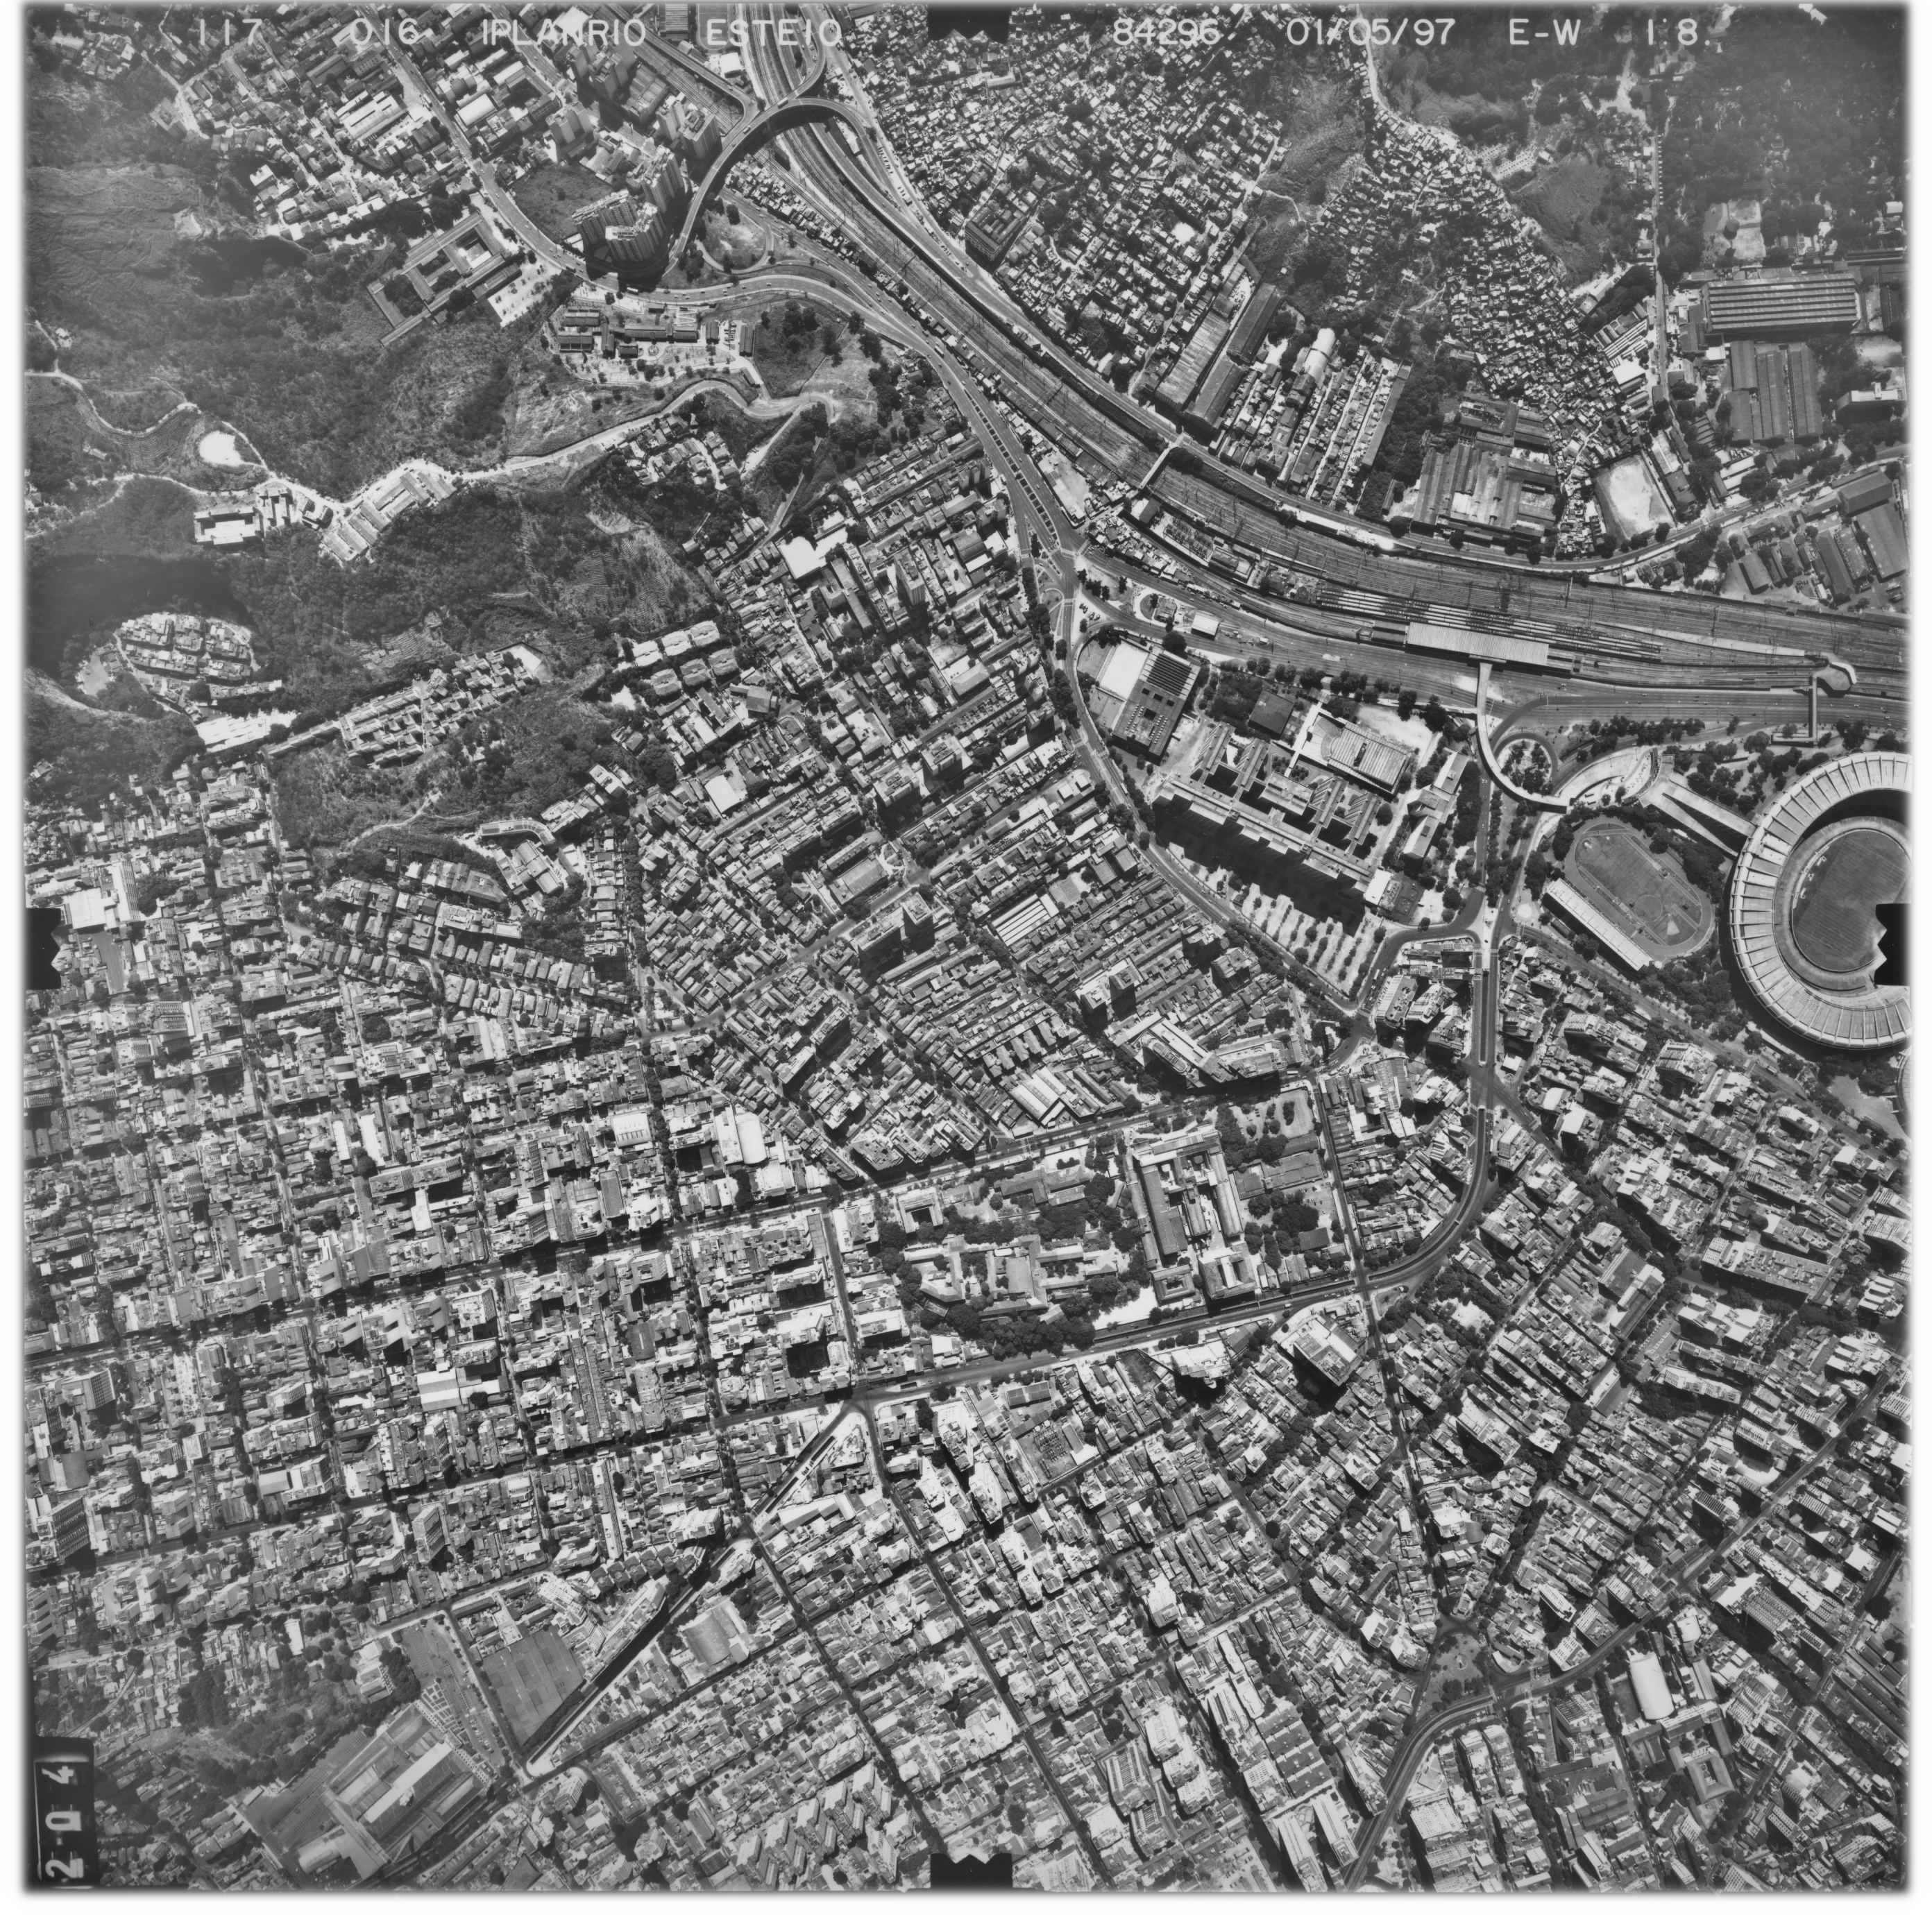
\includegraphics[width=0.3\hsize]{figuras/1997_016_300dpi.png}}}\hfill
  \subfloat[][]{\label{17}
    \setlength{\fboxsep}{0pt}
    \fbox{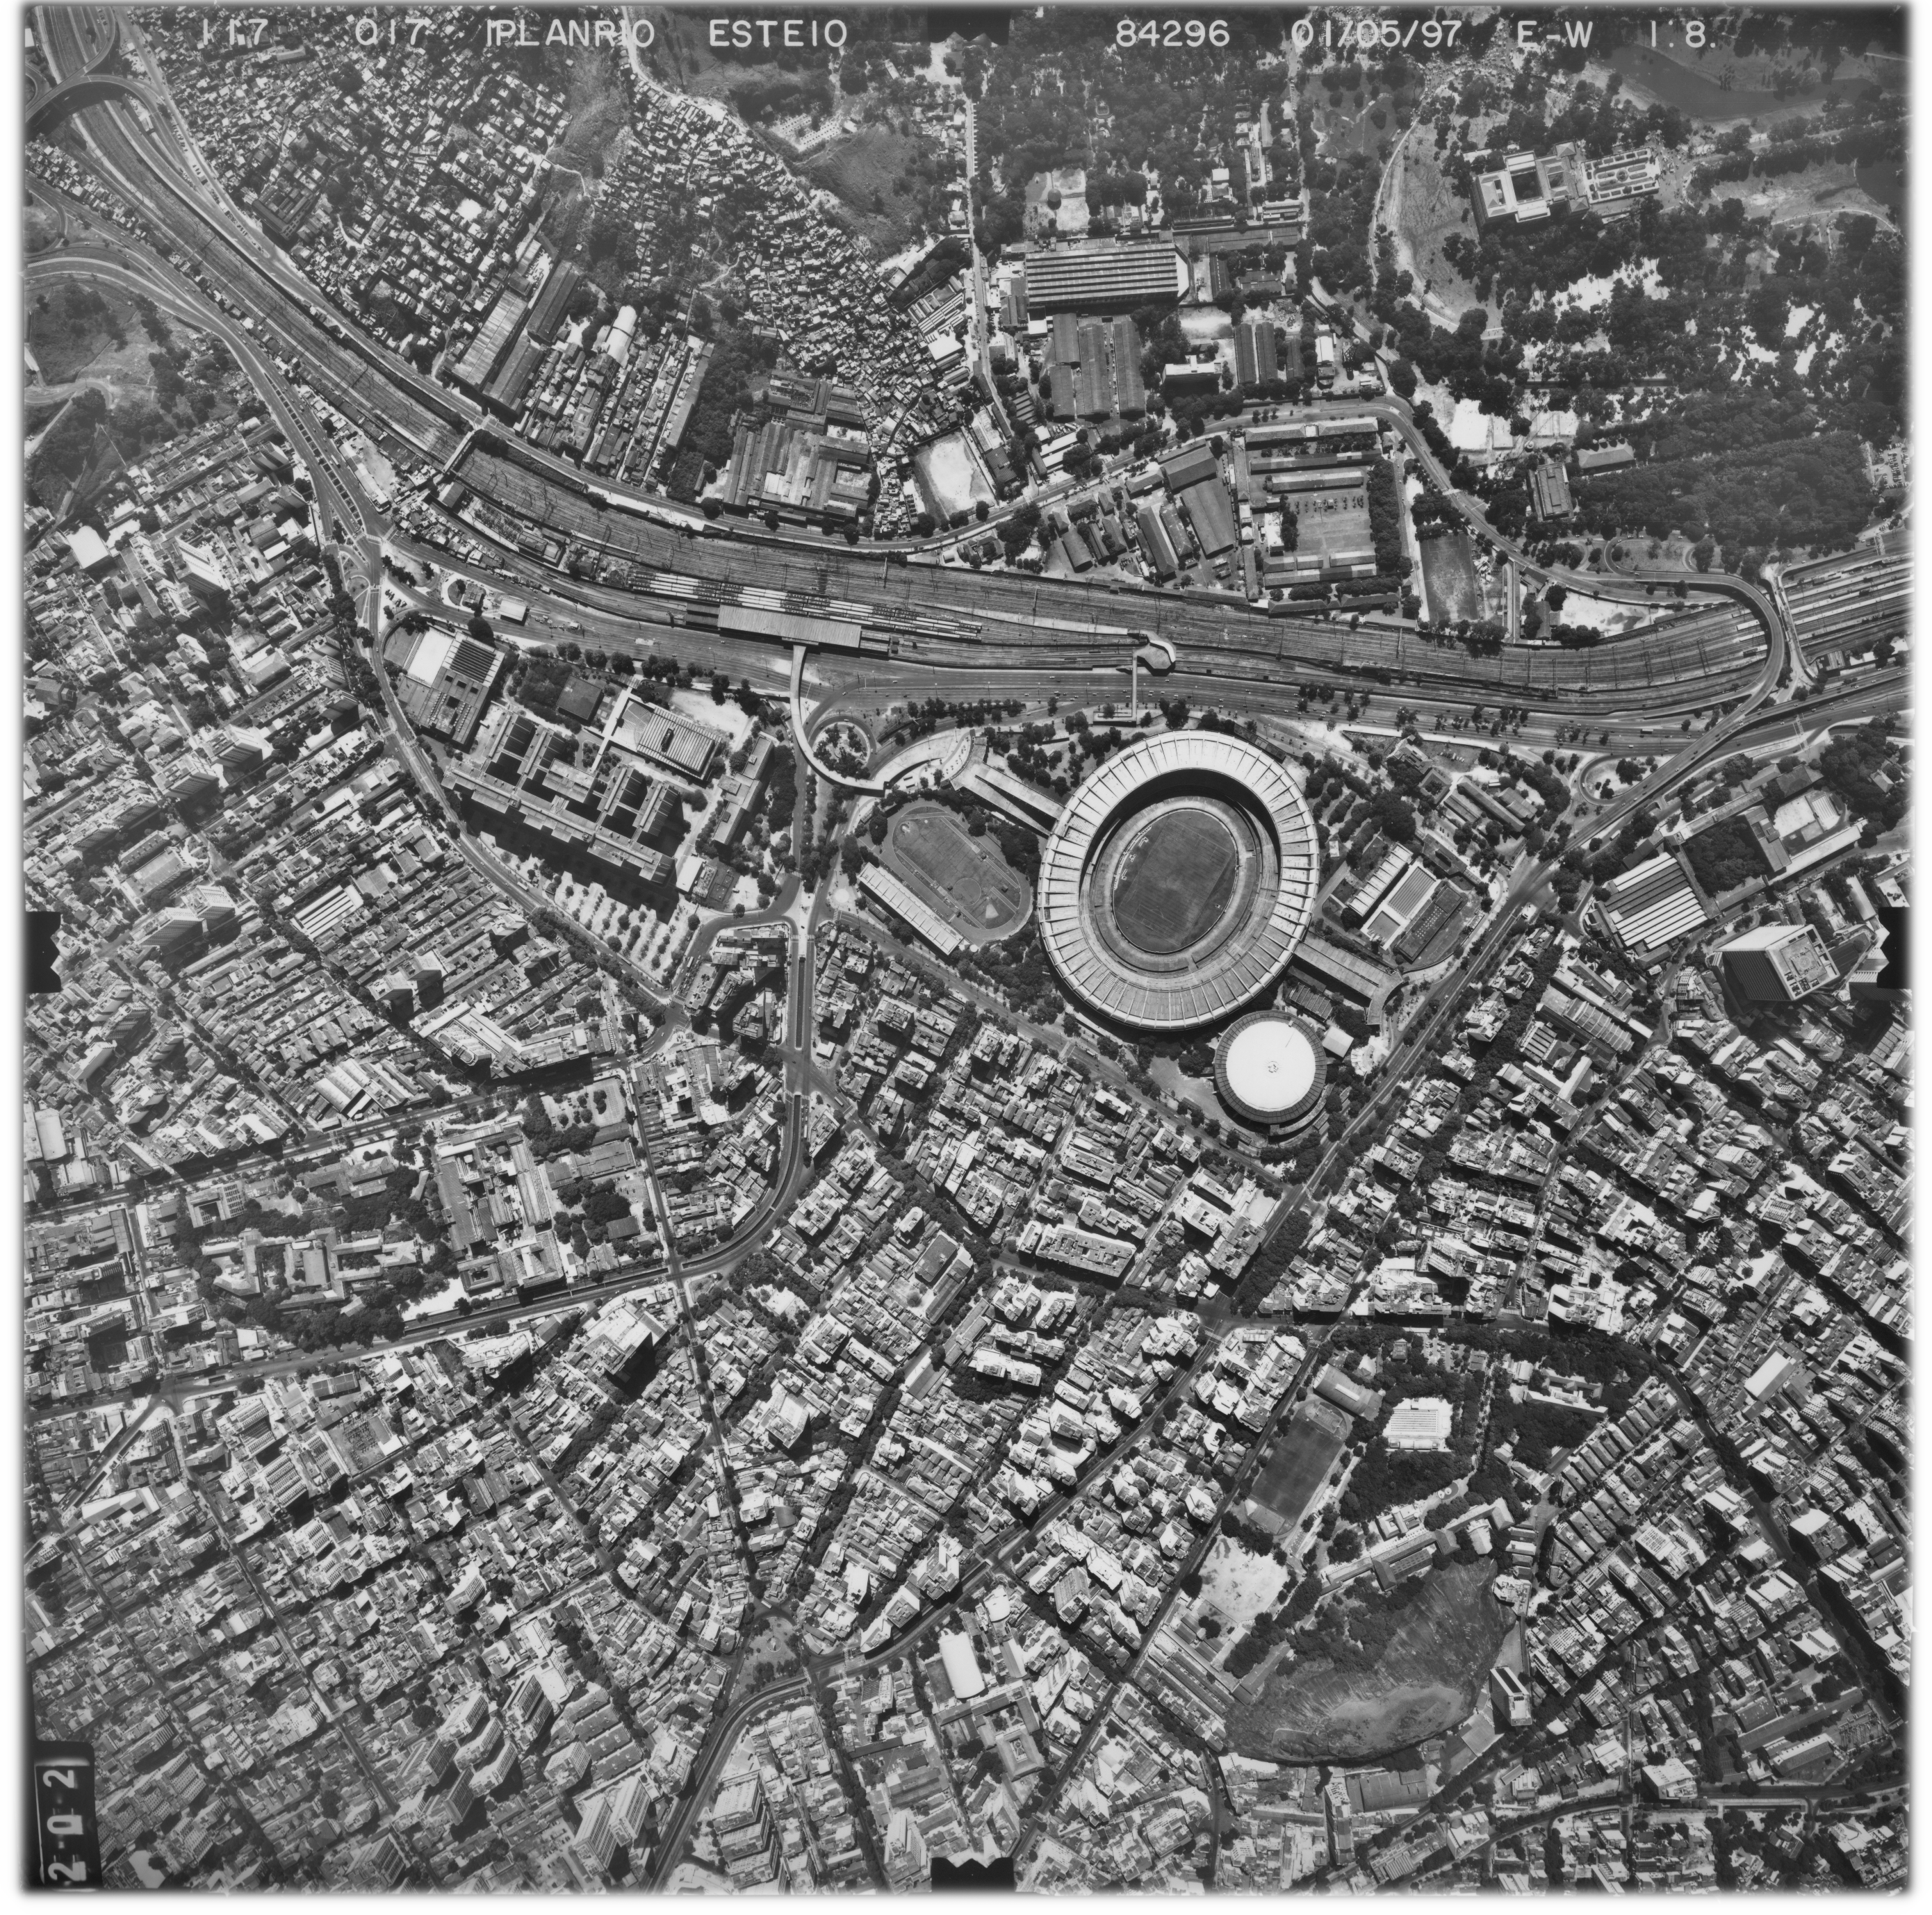
\includegraphics[width=0.3\hsize]{figuras/1997_017_300dpi.png}}}\hfill
  \subfloat[][]{\label{18}
    \setlength{\fboxsep}{0pt}
    \fbox{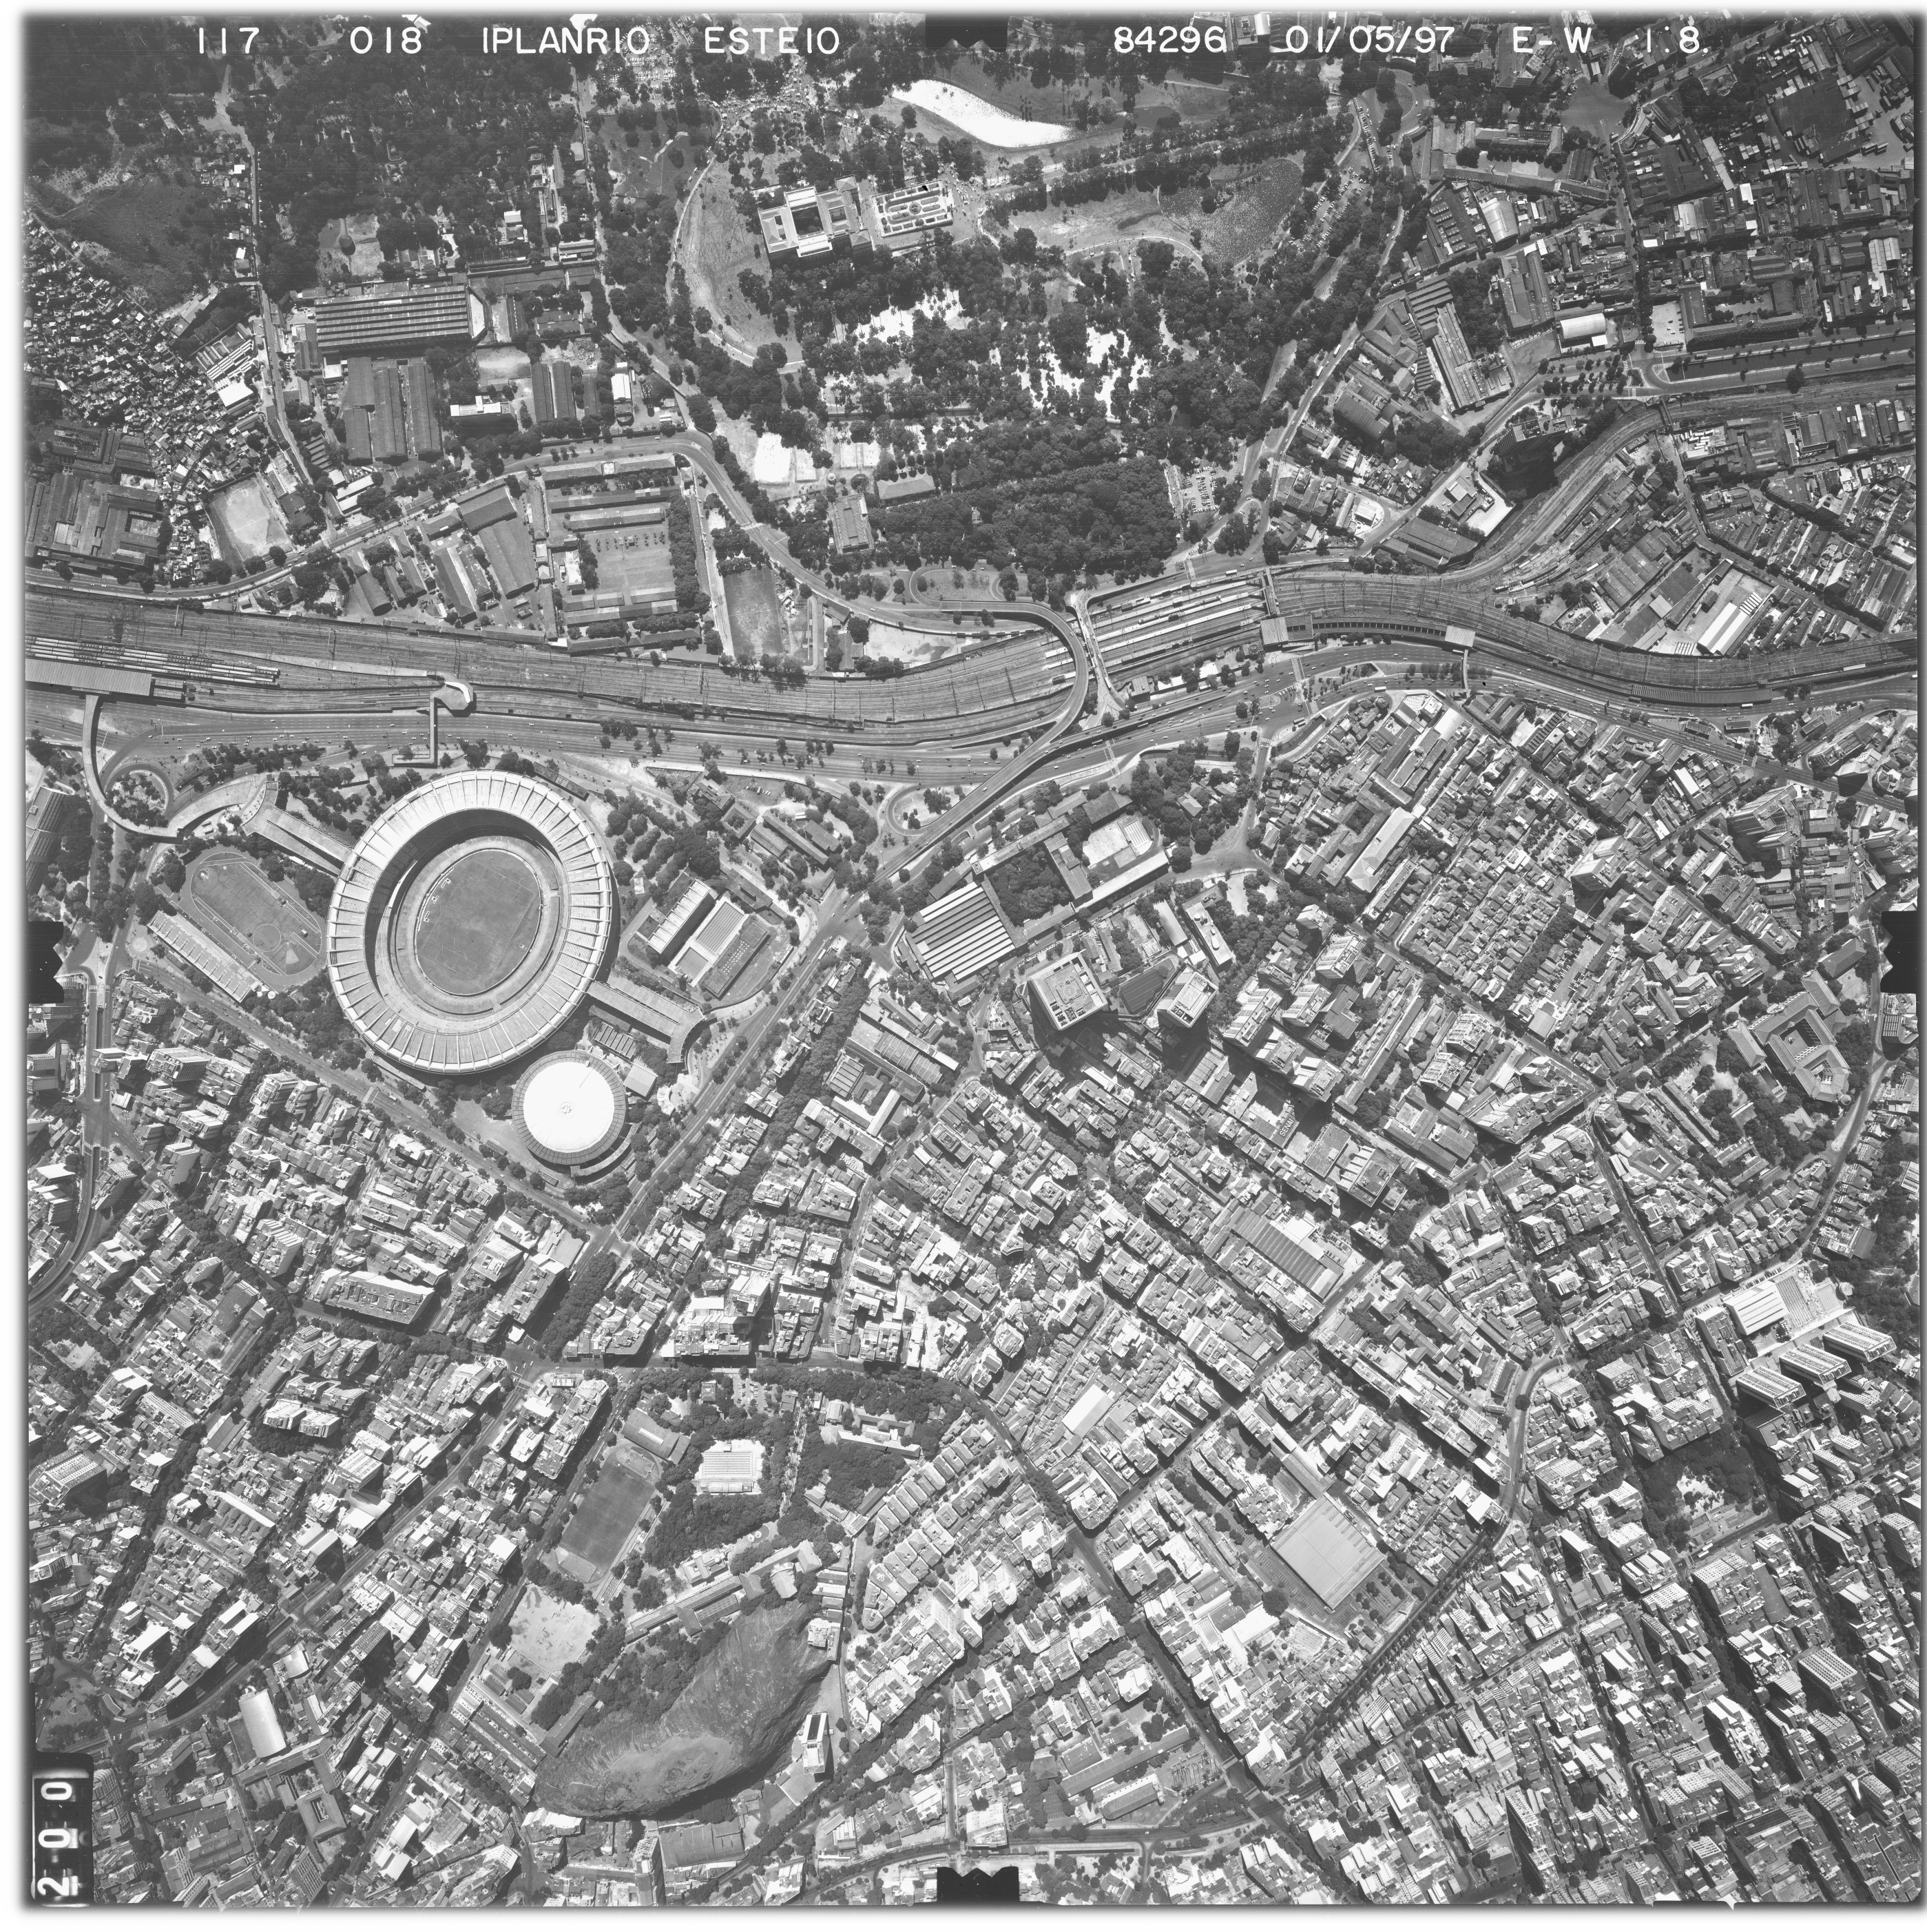
\includegraphics[width=0.3\hsize]{figuras/1997_018_300dpi.png}}}
  \legend{\subref{16} 16;
          \subref{17} 17; e
          \subref{18} 18}
  \source{Arquivo do Projeto E-Foto sobrevoo UERJ de 1997.}
\end{figure}

Um conjunto de imagens de exemplo do e-foto\footnote{O conjunto de imagens pode ser obtido em \url{http://www.efoto.eng.uerj.br/download/imagens-e-dados}}, conforme observado na Figura \ref{16_17_18}, foi adotado nos testes principais deste trabalho. Por simplicidade, estas imagens de sobrevoo da região da Tijuca, com foco na área da UERJ, realizado em 1997 e cedido ao LFSR pelo IPP, serão denominadas 16, 17 e 18 quando exibidas no Capitulo \ref{results}.


\section{Definição dos critérios de análise das opções disponíveis}

Com a fase de estudos finalizada, fez-se indispensável a definição de critérios para comparação entre os métodos disponíveis, tanto para detectar e descrever feições, quanto para compará-las e restringir o conjunto com uma análise geométrica. Estes critérios devem permitir o entendimento de suas diferenças, quantitativas e qualitativas, e como eles se comportariam para imagens de relevância fotogramétrica. Adotaram-se então 4 critérios de análise:

\begin{itemize}
    \item Tempo de execução e memória alocada
    \item Distribuição e volume das respostas
    \item Verificação da qualidade
    \item Viabilidade de filtragem dos melhores pontos
\end{itemize}


\subsection{Tempo de execução e memória alocada}

Para análise do tempo de execução foram isolados pontos específicos dos códigos testados e em desenvolvimento com a biblioteca ``Chrono'', que é parte das bibliotecas nativas do C++11, e adotado retorno de intervalos em milissegundos (ms). Para a quantificação de memória alocada foram feitas macros de cálculo do espaço reservado para as principais estruturas em uso em cada código analisado. Entende-se que a escolha de pontos específicos do processamento, bem como de algumas estruturas principais, não reflete o total de tempo e memória usados. Contudo, é razoável esperar que seja possível averiguar, pela diferença entre as somas obtidas e um contador externo ao programa (como a função \textit{time -v $<$program$>$} do sistema Linux), se as partes selecionadas são realmente as mais significativas de todo o processo.


\subsection{Distribuição e volume das respostas} \label{Dist_gruber}

Este critério implica na percepção visual do preenchimento da região de sobreposição das imagem com pontos correlatos que puderam permanecer até o fim do processo, assim se tornando pontos de costura, bem como do decaimento do número de pontos chaves e de correlações após as etapas de refinamento como a verificação geométrica. Para análise e avaliação da distribuição de respostas será utilizado o conceito de regiões de gruber \cite{manual_photogrammetry}. Tal conceito afirma que apenas quando temos pontos bem distribuídos e de preferência cobrindo distintas regiões de interesse na área de sobreposição das imagens, conforme a ilustra a Figura \ref{gruberarea}, podemos ter uma solução robusta e que elimine a paralaxe vertical.


\begin{figure}[!ht]{12cm}
  \caption{Regiões de interesse para distribuição de pontos de gruber} \label{gruberarea}
  \includegraphics[width=\hsize]{figuras/gruberarea.png}
  %\legend{Texto da legenda.}
  \source{Imagem adaptada de \citeauthoronline{manual_photogrammetry} (\citeyear{manual_photogrammetry})}
\end{figure}
%Para a analise da distribuição de respostas será utilizado o conceito de pontos de gruber 

\subsection{Verificação da qualidade}

Para este critério de análise podem ser considerados tanto a analise visual dos pontos medidos após sua carga no módulo de aerotriangulação ou numa imagem do par, quanto o valor numérico de erro quando usamos uma transformação projetiva (homografia) para projetar pontos de uma imagem sobre a outra na qual há correlatos previamente estimados. 

\subsection{Viabilidade de filtragem de melhores pontos}

A viabilidade de filtragem dos melhores pontos serve ao princípio de não sobrecarregar o projeto com pontos. Logo, é importante que parâmetros adicionais possam ser adotados na solução final para efetuar controle do total de pontos gerados.



\section{Planejamento de testes comparativos}

Para verificar a viabilidade de execução de todos os algoritmos selecionados foram localizadas bases comuns de código, principalmente entre os exemplos do módulo \textit{features2d}\footnote{Materiais disponíveis em \url{https://docs.opencv.org/4.5.4/d9/d97/tutorial_table_of_content_features2d.html}}. 
Os exemplos para estudo deste módulo incluem a produção e uso de detectores, bem como a apresentação de diferentes extratores de feições, métodos de correlação e a verificação geométrica, incluindo a aplicação na localização de objetos em imagens e de rastreamento em vídeo.
Foram então planejados e efetuados testes de configuração com os diferentes algoritmos em estudo adotando-se um mesmo fluxo de base. Foram incorporadas e testadas diferentes técnicas de tomada de medidas para extrair os valores que atendessem aos critérios definidos. Ao fim deste planejamento, foi possível esboçar um conjunto de variações nas entradas que pudessem ser usadas para testar o produto final.



\section{Codificação da solução}

Tendo feito modificações e testes de uso de diversos exemplos de código da biblioteca, iniciou-se a fase de codificação de um produto final (disponível no Apêndice \ref{codigofonte}) integrando aspectos estudados para atender o objetivo deste projeto. Por simplificação foi adotada a interface de linha de comandos, entendendo que esta poderá ser acessada diretamente por outro software, como o e-foto, para obter os pontos de costura dado um conjunto de argumentos variado.

\begin{figure}[!h]{15cm}
  \caption{Fases da execução da solução de linha de comando proposta} \label{macro}
  \includegraphics[width=\hsize]{figuras/macro.png}
  %\legend{}
  \source{O autor}
\end{figure}

De um ponto de vista geral, as partes do processo podem ser descritas como indica a Figura \ref{macro}, onde é observado que além do processamento principal é  a necessidade de ao menos duas fases dedicadas à interface com o mundo externo. A interpretação dos argumentos lida com informações de entrada que configuram o pedido de processamento. A persistência de resultados lida com a saída das respostas encontradas durante o processo principal. Ao seu tempo, o processo principal pode ser subdividido em 3 outros focados em tratamento das imagens individualmente, dos pares sugeridos pelo usuário e das medidas identificadas pelo processamento de pares.

Por sua vez, as tentativas de acomodar a solução com programação procedural apenas, como transcorre na maioria dos exemplos de OpenCV, mostrou-se de grande complexidade para a documentação, pois muitas em alguns pontos o código tornava-se de difícil leitura. Por exemplo, assumindo que uma função \textit{knnMatch} pode retornar os $n$ vizinhos mais próximos de cada um dos $m$ pontos chaves descritos, e que este processo seria repetido $p$ vezes para atender aos pares processados, 
teríamos um vetor com 3 dimensões causando uma complexa administração de índices ao acessar tais informações, ou seja, algo como \textit{knnResult[i][j][k]} seria necessário para indicar o k-ésimo vizinho do j-ésimo ponto chave da primeira imagem do i-ésimo par de imagens.

\begin{figure}[!h]{16cm}
  \caption{Diagrama de classe da solução} \label{classdiagram}
  \includegraphics[width=\hsize]{figuras/classdiagram.png}
  %\legend{}
  \source{O autor}
\end{figure}

Pela adoção de um modelo de programação orientado à objetos podemos ainda expressar a estrutura da solução proposta em termos de linguagem gráfica na notação UML, conforme ilustra a Figura \ref{classdiagram}. No diagrama de classes um controlador de processo define métodos para as principais atividades, além de um método de impressão dos argumentos para uso da solução. O controlador de processo acomoda todas as imagens carregadas através do arquivo de entrada, instancia os pares cuidando das ligações necessárias com suas imagens (evitando assim a repetição das informações de imagens em memória) e cria, atualiza ou junta pontos durante o processamento de medidas (haja visto que pontos de costura precisam ser medidos em diferentes imagens). No processamento de pares e imagens, o controlador repete a chamada de métodos apropriados de cada imagem a ser descrita ou par a ser correlacionado. 

Objetos de OpenCV que configuram pontos chaves e correlações, bem como matrizes de descrição ou transformações geométricas, são apresentados no diagrama de classe e cabe notar que a OpenCV usa índices numéricos (ligações indiretas) que apontam estes objetos pela posição em que se encontram num \textit{container} de dados, tipicamente vetores da biblioteca padrão de C++, a STL (acrônimo para \textit{Standard Template Library} ou biblioteca de modelos padrão). 

A ligação entre as classes imagem e ponto faz-se importante em dois momentos e nos dois sentidos, sendo caracterizada a ligação com o ponto, isto é, partindo da imagem, como prioritária. Isto se justifica pelo algoritmo de integração da medidas dos pontos de costura quando estes ocorrem em pares distintos. Nos casos onde uma imagem participa de diversos pares é necessária a busca na imagem pela medida, a fim de determinar se esta já foi registrada durante o processamento de outros pares com a mesma imagem. Ao seu tempo, a ligação com a imagem, partindo do ponto, faz-se necessária em termos de entrega do produto final, na qual cada medida do ponto em distintas imagens deve ser corretamente associada. A associação das medidas de cada ponto podem então ser atendidas com uma simples cópia do índice da imagem, sem que isso implique em perda de performance ou grande consumo de memória.



\subsection{Escolha de argumentos}

Para possibilitar alguma flexibilidade de uso, a solução final requer que sejam apontados nomes de arquivos de entrada e sugeridos outros dois nomes para os arquivos de saída. Além destes arquivos, é possível adicionar opções de configuração que podem, entre outras coisas, trocar o método de detecção e descrição em uso, alternar entre os métodos de correlação disponíveis e inserir critérios para limitar o conjunto de resultados obtidos.

O primeiro dos arquivos de entrada esperados é uma lista de caminhos para as imagens que serão processadas, precedidas de seus índices no projeto, pois o resultado será apresentado em termos destes índices de imagens. O segundo arquivo deve indicar quais pares de imagens devem ser processados. Neste segundo arquivo, apenas os índices de imagens precisam ser apresentados.

Alternativamente, uma opção \textit{mode} pode ser usada para escolher processar todos os pares possíveis (\textit{ALL}) ou através da sequência (\textit{SEQUENCE}), na qual as imagens foram descritas. Deste modo, se \textit{SEQUENCE} está ativo e as imagens listadas são 16, 17 e 18, por exemplo, os pares serão 16 com 17 e 17 com 18.

Já os nomes dos arquivos de saída devem ser indicados para que sejam gravados, no primeiro arquivo, as medidas nas imagens para cada ponto de costura, e no segundo arquivo, o índice e tipo de cada ponto. Neste segundo arquivo são gravados então o tipo \textit{Photogrammetric}, que indicam para o e-foto que estes podem ser usados na aerotriangulação, e uma sequência com 6 zeros (valores para E, N, H e suas precisões destas 3 medidas, quando disponíveis). A gravação com zeros é feita para que o e-foto não precise de quaisquer alterações evitando assim erros de leitura. Cabe notar que no processo de aerotriangulação as coordenadas de mundo destes pontos serão sobrescritas.

Na versão 472\footnote{Método disponível em \url{https://sourceforge.net/p/e-foto/code/472/tree/trunk/qt/interface/ProjectUserInterface\_Qt.cpp\#l2635}} do código do e-foto, observou-se que o método \textit{importPointsFromTxt2} pode ser acessado somente pelo atalho de teclado (``Ctrl+Shift+P''). Este está disponível durante a execução do módulo de projetos e resulta no pedido de dois arquivos a saber: arquivo de coordenadas ENH (nossa segunda saída); e o arquivo de medidas no espaço das imagens.

Argumentos extras para o processamento incluem:

\begin{itemize}
    \item \textbf{detector} para selecionar o algoritmo adotado (AKAZE, ORB, SIFT ou SURF);
    \item \textbf{ccheck} para acionar a verificação cruzada de correlações com BFM (desligando o FLANN);
    \item \textbf{verbose} para ligar a impressão de informações do processamento úteis na confecção dos resultados apresentados no Capítulo \ref{results};
    \item \textbf{number\_f} para definir o número $f$ de pontos chaves o algoritmo ORB irá detectar;
    \item \textbf{force\_f} para ativar a limitação de detecções nos demais algoritmos baseado em $f$;
    \item \textbf{gruber\_roi} para ativar a limitação da área passível a detecção de pontos chave;
    \item \textbf{help} para exibir os parâmetros e suas descrições;
    \item \textbf{init\_index} para definir o identificador inicial dos pontos de costura;
    \item \textbf{list\_pairs} para registrar os pares que possuem solução com uma taxa de \textit{inliers} desejada;
    \item \textbf{limit\_out} para limitar a saída de pontos de costura por par;
    \item \textbf{mode} para definição do modo em que serão selecionados os pares;
    \item \textbf{n\_measures} para limitar os pontos àqueles contidos em um mínimo de $n$ imagens;
    \item \textbf{residue} para definir o valor máximo do resíduo aceito na verificação geométrica;
    \item \textbf{scale} para definir o denominador para realizar a redução das imagens;
\end{itemize}

A impressão de toda a lista de argumentos foi programada para atender a opção \textit{help}, ou no caso de quaisquer falhas de execução do processo que inviabilizem a gravação de resultados. Erros graves que podem suspender o processamento geram mensagens ao usuário, como a inviabilidade de abrir uma das imagens indicadas pelo usuário, enquanto que falhas toleráveis, como a inviabilidade de obter medidas para um par, são contornadas e podem ser reportadas ao final do processo.



\subsection{Processamento de imagens}

No processamento de imagens se cumprem as extrações dos pontos chaves do conjunto de imagens. Há método em OpenCV para fazê-lo para um conjunto de imagens pré-carregadas pelo usuário, contudo entende-se que se o tamanho de todas as imagens for muito grande pode ser inviável usar este recurso. Logo, como indicado na Figura \ref{fl:imagens}, adotou-se uma sequência de atividades onde cada imagem é aberta, tem suas informações extraídas e então fechada, tendo o número de pontos-chave relatado se solicitado. 

\begin{figure}[!h]{15cm}
  \caption{Diagrama de atividades para o processamento de imagens} \label{fl:imagens}
  \includegraphics[width=\hsize]{figuras/Fluxo_Imagem.png}
  %\legend{}
  \source{O autor}
\end{figure}

De igual modo, os exemplos disponibilizados pela OpenCV demonstram a detecção e descrição simultaneamente, porém optamos por separar essas atividades para que uma melhor compreensão dos algoritmos possa ser alcançada. Isto ajuda na quantificação de tempos individuais para estas etapas e poderia ser usado para mesclar os métodos ou adotar algoritmos especializados em uma das duas atividades. Medidas de tamanho das estruturas podem demonstrar como o processo escala em memória e ajudam a compreender qual a quantidade de memória que pode vir a ser necessária para grandes conjuntos de imagens com cada método.



\subsection{Processamento de pares}

O processamento de pares faz correlação de pontos chaves descritos previamente para as imagens e, em seguida, verifica se é possível obter uma solução de transformação geométrica entre o conjunto de pares, considerando um erro máximo de reprojeção aceitável. Estas atividades são implementadas integralmente pela OpenCV, mas é importante realizarmos atividades extras, como as ilustradas na Figura \ref{fl:pares}, para selecionar melhores correlações e registrar os erros de medida observados. Estes erros são possíveis de computar usando a transformação geométrica, que restringe os pontos da solução final.

\begin{figure}[!h]{15cm}
  \caption{Diagrama de atividades para o processamento de pares} \label{fl:pares}
  \includegraphics[width=\hsize]{figuras/fluxo_pares.png}
  %\legend{}
  \source{O autor}
\end{figure}

A correlação dos pontos chaves pode ser feita por força bruta (BFMatcher na OpenCV), isto é, cada ponto chave em uma imagem é confrontado com todos os pontos chaves da outra imagem no par. Deste modo, são preservadas as menores distâncias no espaço de descrição observadas para cada ponto chave processado. Embora caro computacionalmente, ficando seu uso restrito aos pequenos conjuntos de dados, este processo permite a verificação cruzada de vizinhos mais próximos. Isto equivale a responder a questão ``se um ponto chave $P$, na primeira imagem, possui melhor correlação com um ponto chave $Q$, na segunda imagem, a análise no sentido oposto também é verdadeira?'', onde o ``afirmativo'' corresponde a correlação cruzada.

A alternativa viável ao processamento de correlações por força bruta, quando o conjunto de pontos chaves é muito grande, é a busca por vizinhos mais próximos aproximados (FlannBasedMatcher na OpenCV). Ela usa estruturas especializadas para a busca espacial, como as árvores de k-dimensões (KD-Tree) ou o hash sensível à localidade (LSH), implementadas e amplamente divulgadas pela biblioteca flann\footnote{\textit{Fast Library for Approximate Nearest Neighbors} está disponível em \url{https://github.com/flann-lib/flann}}. Neste caso, a estrutura de busca espacial deve estar alinhada ao descritor usado, ou seja, descritores binários requerem algoritmos de hash, enquanto descritores modelados com números reais, como SIFT e SURF, usam KD-Tree. Esta diferença é notável na própria forma de computar distâncias, pois a distância aplicável aos descritores binários é a distância de Hamming \cite{ORB}.

O ganho em tempo de execução quando utilizados vizinhos mais próximos aproximados é contraposto pela inviabilidade de verificação cruzada. Contudo, um outro critério de eliminação pode ser adotado ao observar a razão entre a distância para o vizinho mais próximo de um ponto chave e o segundo vizinho mais próximo. A lógica embarcada nesta observação é que um ponto chave com apenas um vizinho mais próximo é potencialmente mais relevante do que aqueles que possuem mais de um vizinho em seu entorno \cite{SIFT2004}.

É importante notar que apenas selecionar as melhores correlações pode não ser suficiente para eliminar erros grosseiros. Logo, uma segunda rodada de análise, considerando as restrições geométricas que podem ser observadas para imagens de uma mesma cena, deve ser aplicada. Nesta atividade, um outro módulo de OpenCV, \textit{calib3d}, apresenta contribuições importantes, das quais adotamos o método \textit{findHomography}. Sua aplicação principal é o cálculo de uma transformação projetiva entre os planos das imagens dadas por um conjunto de pontos correlatos. Aqui aplicam-se as técnicas de ajustamento robustas discutidas anteriormente e, como consequência, podem ser identificados e removidos quaisquer pares de pontos chaves que apresentem erro de reprojeção superior a algum limiar definido pelo usuário.

De posse da transformação geométrica podemos ainda registrar e classificar as correlações restantes segundo o resíduo observado. Entendemos que este pode ser um critério melhor do que a distância de correlação propriamente quando se trata da seleção dos melhores pontos de costura para um bloco de imagens.



\subsection{Processamento de medidas}

Com os dados obtidos após o processamento de pares, resta a organização das medidas a serem salvas como resultado do processo. Isto é feito pelo próprio controlador de processo, tendo em vista que ele é o detentor de todas as informações e que os pontos de costura individualmente não devem realizar qualquer processamento, além do registro de suas medidas, evitando indexar a mesma imagem mais de uma vez. 

Embora seja viável na OpenCV correlacionar feições de uma imagem com diversas outras em apenas uma chamada, algo que se aplica muito bem para aplicações de detecção de objetos, esta abordagem parece inapropriada para a finalidade de costura de blocos fotogramétricos, pois tornar-se-ia complexo distinguir entre padrões repetitivos de bons pontos de costura observáveis em mais de duas imagens. Porém, para o e-foto e para a fotogrametria em geral, uma faixa de aerofotos pode ter inúmeras imagens, todas com sobreposição regular e muitas faixas, onde a sobreposição é menor, mas pode haver boas feições. Logo, é desejável a percepção de pontos em 3 ou mais imagens, mesmo se considerarmos apenas uma faixa com recobrimento lateral de aproximadamente 60\%, que é o caso da maioria das faixas de sobrevoo convencionais. Para mais, aerolevantamentos com drones podem ter ainda mais sobreposição para compensar os pequenos formatos de sensores e a falta de estabilidade destas plataformas. 

Logo, julgamos que não cabe registrar todos os pares de pontos correlatos diretamente sem antes efetuar qualquer crítica sobre a possibilidade de um mesmo ponto chave ser bem correlacionado, e com pouco resíduo, em diferentes pares de imagens. O que se espera obter é a observação de uma propriedade transitiva que afirma, ``Se $a=b$ e $b=c$, então $a=c$'', ou seja, pela correlação ter sido realizada em imagens par-a-par, um mesmo ponto pode estar em dois ou mais pares e ter algumas de suas coordenadas ligadas a duas outras imagens ou mais. Uma extensão da mesma propriedade pode ser importante para lidar com o encadeamento não sequencial de pares, isto é, ``Se $a=b$, $c=d$ e posteriormente é constatado que $b=c$, então $a=c$, $a=d$ e $b=d$''.

\begin{figure}[!h]{15cm}
  \caption{Diagrama de atividades para o processamento de medidas} \label{fl:medidas}
  \includegraphics[width=\hsize]{figuras/fluxo_medidas.png}
  %\legend{}
  \source{O autor}
\end{figure}

Com o entendimento destas possibilidades de combinação de pares podemos formular um diagrama de atividades que incorpore a criação, atualização e fusão de pontos chaves, como o ilustrado na Figura \ref{fl:medidas}. Então para todos os \textit{inliers} de cada par repete-se o processo de registro das medidas observadas. A criação de um novo ponto de costura ocorre sempre que nenhuma das imagens do par registrou previamente a medida observada. Se apenas uma delas registrou o previamente a medida observada, então existe um ponto de costura a ser atualizado pela adição de mais uma medida. Contudo, se ambas as imagens de um par já registraram as medidas observadas, pode haver dois pontos de costura distintos que se aplicam a uma mesma feição do espaço objeto. Neste caso, as medidas devem ser mescladas num único pontos de costura. 

Para a busca na imagem por medida pré-existente adotou-se a estrutura de dados \textit{map}\footnote{Ajustes necessários para uso desta estrutura com os pontos do OpenCV foram indicados em \url{https://stackoverflow.com/questions/26483306/stdmap-with-cvpoint-as-key}} da STL, pois esta possui tempo de acesso reduzido, aplicando internamente o algoritmo de busca binária. Outras alternativas seriam adotar uma \textit{KD-tree}, com tempo de acesso equivalente ao \textit{map}, ou um algoritmo de \textit{hash} (como implementado em \textit{unordered\_map}) com tempo de resposta menor, mas possivelmente com elevado custo de armazenamento.


\subsection{Persistência de dados}

A persistência de dados será realizada sob os formatos de arquivos adotados pelo método de inserção pré-existente no e-foto. O primeiro arquivo solicitado pelo e-foto identifica o ponto, atribui um tipo e apresenta os valores para E, N e H e as precisões deste no espaço objeto. Assim, para cada ponto de costura gerado teremos uma linha, como pode ser observado na Figura \ref{exemp_ENH}, onde o primeiro valor equivale à identificação do ponto seguido pelo tipo de ponto. Os demais valores são zerados, pois não se aplicam aos pontos fotogramétricos. 

\begin{figure}[!ht]{12cm}
  \caption{Exemplo do arquivo de persistência de pontos.} \label{exemp_ENH}
  \fbox{\includegraphics[width=\hsize]{figuras/exemplo_ENH.png}}
  \legend{Da esquerda para a direita as colunas representam: identificação de cada ponto; tipo de ponto; E; N; H; e suas respectivas precisões.}
  \source{O autor.}
\end{figure}

\begin{figure}[!ht]{12cm}
  \caption{Exemplo do arquivo de persistência de medidas.} \label{Exemp_saida}
  \subfloat[][]{\label{saida1}
    \fbox{\includegraphics[width=0.45\hsize]{figuras/exemplo_saida1.png}}}\hfill
  \subfloat[][]{\label{saida2}
    \fbox{\includegraphics[width=0.45\hsize]{figuras/exemplo_saida.png}}}\\
  \legend{Da esquerda para a direita as colunas representam: índice na imagem; índice do ponto; coluna; e linha de medição do ponto na imagem.\\
  \subref{saida1} Medidas dos pontos de índice 462 à 466; e\\
  \subref{saida2} Medidas dos pontos de índice 467 à 470.}
  \source{O autor.}
\end{figure}

Por sua vez, a Figura \ref{Exemp_saida} ilustra o conteúdo do segundo arquivo solicitado, no mesmo processo de importação de pontos fotogramétricos pelo e-foto. Este arquivo leva as medidas dos pontos em coordenadas digitais (no espaço imagem) a serem inseridas. Quatro colunas são usadas para: a identificação da imagem na qual o ponto foi medido; indexar do ponto medido; e transmitir as coordenadas em coluna e linha, respectivamente. 

Cabe destacar que a carga de pontos fotogramétricos no e-foto poderia ainda ser modificada para eliminar a necessidade do arquivo que identifica o ponto, pois este não agrega qualquer informação que não possa ser derivada do segundo formato de arquivo solicitado. Por este motivo o fornecimento de nome para arquivo que identifica os pontos é considerado opcional na solução proposta. Restando o nome do arquivo de medidas nas imagens como argumento obrigatório na interface de linha de comando definida. Este mesmo arquivo é preenchido de forma distinta apenas quando a opção \textit{list\_pairs} está ativa, de modo que podem ser gravados os índices de cada par que possuem solução com uma taxa de \textit{inliers} estipulada pelo usuário.

Como a exibição dos pontos importados no e-foto se dá através de listas de pontos ou pela plotagem sobre o par de imagens na execução da fototriangulação pode ser trabalhoso conferir pontos que possuem medidas em 3 ou mais imagens. Por este motivo, recomenda-se a criação futura de um módulo para exibir e manipular o foto-índice do projeto. Tal módulo vindouro poderia adicionar recursos para melhor gerenciamento de grandes volumes de dados permitindo, por exemplo, a ocultação de pontos que atendam a algum critério de filtragem.

%=====================================================================
\chapter{Resultados}\label{results}
%==================================================================

Neste capítulo serão apresentados alguns dos resultados obtidos para os diversos testes realizados durante a execução desse projeto. Inicialmente serão apresentados valores numéricos e avaliadas as diferenças entre algoritmos adotados, na sequência serão ilustrados os resultados sobre pares de imagens para a conferência visual das correlações e finalmente serão consideradas as variações que podem ser obtidas pela manipulação dos argumentos admitidos na solução construída. 

\section{Resultados numéricos dos testes}

Após codificação do produto final e execução dos testes planejados temos resultados divididos entre subprocessos de imagens, que realiza detecção e descrição de feições; de pares de imagens, que implicam nas correlações e verificações geométricas; e de medidas, que implicam em sumarizar os pontos de costura obtidos.

\subsection{Custo de detecção e descrição}

A apresentação dos resultados foi realizada através da Tabela \ref{Det&Dec} por imagem e, para maior clareza, foram agrupados para cada algoritmo seus tempos de detecção de feições, número de respostas obtidas, uma razão entre esses valores e o espaço de memória alocado em MB (\textit{Mega Byte}) para a resposta. Também foram integrados dados de tempo da descrição de feições e uma razão entre este e o número de feições, além do espaço necessário para manter a descrição disponível para as etapas seguintes no fluxo da aplicação. A última coluna da mesma tabela apresenta médias dos valores anteriores de cada imagem para auxílio na análise.

\begin{table}[!ht]{15,5cm}
\caption{Resultados numéricos de detecção e descrição dos métodos analisados.}\label{Det&Dec}
\begin{tabular}{c|c|c|ccc|c}
\hline
\multirow{2}{*}{Método} & \multirow{2}{*}{Etapa} & \multirow{2}{*}{Medida} & \multicolumn{3}{c|}{Imagens} & \multirow{2}{*}{Média} \\ \cline{4-6}
 &  &  & \multicolumn{1}{c|}{16} & \multicolumn{1}{c|}{17} & 18 &  \\ \specialrule{.1em}{.05em}{.05em}
\multirow{7}{*}{AKaze} & \multirow{4}{*}{Detecção} & Número   de pontos & \multicolumn{1}{c|}{81652} & \multicolumn{1}{c|}{78797} & 73851 & 78100 \\ \cline{3-7} 
 &  & Tempo total   (ms) & \multicolumn{1}{c|}{1208,4} & \multicolumn{1}{c|}{974,291} & 899,603 & 1027,431 \\ \cline{3-7} 
 &  & Tempo / Ponto & \multicolumn{1}{c|}{0,015} & \multicolumn{1}{c|}{0,012} & 0,012 & 0,013 \\ \cline{3-7} 
 &  & Tamanho alocado(MB) & \multicolumn{1}{c|}{2,170} & \multicolumn{1}{c|}{2,100} & 1,970 & 2,080 \\ \cline{2-7} 
 & \multirow{3}{*}{Descrição} & Tempo total (ms) & \multicolumn{1}{c|}{1138,68} & \multicolumn{1}{c|}{1029,09} & 967,404 & 1045,058 \\ \cline{3-7} 
 &  & Tempo / Ponto & \multicolumn{1}{c|}{0,014} & \multicolumn{1}{c|}{0,013} & 0,013 & 0,013 \\ \cline{3-7} 
 &  & Tamanho alocado(MB) & \multicolumn{1}{c|}{19,000} & \multicolumn{1}{c|}{18,330} & 17,180 & 18,170 \\ \specialrule{.1em}{.05em}{.05em} %\hline
\multirow{7}{*}{ORB} & \multirow{4}{*}{Detecção} & Número de   pontos & \multicolumn{1}{c|}{100000} & \multicolumn{1}{c|}{100000} & 100000 & 100000 \\ \cline{3-7} 
 &  & Tempo total   (ms) & \multicolumn{1}{c|}{302,914} & \multicolumn{1}{c|}{261,936} & 267,354 & 277,401 \\ \cline{3-7} 
 &  & Tempo / Ponto & \multicolumn{1}{c|}{0,003} & \multicolumn{1}{c|}{0,003} & 0,003 & 0,003 \\ \cline{3-7} 
 &  & Tamanho alocado(MB) & \multicolumn{1}{c|}{2,660} & \multicolumn{1}{c|}{2,660} & 2,660 & 2,660 \\ \cline{2-7} 
 & \multirow{3}{*}{Descrição} & Tempo total (ms) & \multicolumn{1}{c|}{192,903} & \multicolumn{1}{c|}{203,595} & 190,662 & 195,72 \\ \cline{3-7} 
 &  & Tempo / Ponto & \multicolumn{1}{c|}{0,0019} & \multicolumn{1}{c|}{0,0020} & 0,0019 & 0,002 \\ \cline{3-7} 
 &  & Tamanho alocado(MB) & \multicolumn{1}{c|}{12,2} & \multicolumn{1}{c|}{12,2} & 12,2 & 12,2 \\ \specialrule{.1em}{.05em}{.05em} %\hline
\multirow{7}{*}{SIFT} & \multirow{4}{*}{Detecção} & Número de   pontos & \multicolumn{1}{c|}{114684} & \multicolumn{1}{c|}{106728} & 103486 & 108299 \\ \cline{3-7} 
 &  & Tempo total   (ms) & \multicolumn{1}{c|}{2252,18} & \multicolumn{1}{c|}{1823,36} & 1589,33 & 1888,29 \\ \cline{3-7} 
 &  & Tempo / Ponto & \multicolumn{1}{c|}{0,02} & \multicolumn{1}{c|}{0,017} & 0,015 & 0,017 \\ \cline{3-7} 
 &  & Tamanho alocado(MB) & \multicolumn{1}{c|}{3,06} & \multicolumn{1}{c|}{2,84} & 2,76 & 2,887 \\ \cline{2-7} 
 & \multirow{3}{*}{Descrição} & Tempo total (ms) & \multicolumn{1}{c|}{2496,85} & \multicolumn{1}{c|}{2382,41} & 2244,64 & 2374,633 \\ \cline{3-7} 
 &  & Tempo / Ponto & \multicolumn{1}{c|}{0,022} & \multicolumn{1}{c|}{0,022} & 0,022 & 0,022 \\ \cline{3-7} 
 &  & Tamanho alocado(MB) & \multicolumn{1}{c|}{55,99} & \multicolumn{1}{c|}{52,11} & 50,53 & 52,877 \\ \specialrule{.1em}{.05em}{.05em} %\hline
\multirow{7}{*}{SURF} & \multirow{4}{*}{Detecção} & Número de   pontos & \multicolumn{1}{c|}{91048} & \multicolumn{1}{c|}{90826} & 104511 & 95462 \\ \cline{3-7} 
 &  & Tempo total   (ms) & \multicolumn{1}{c|}{1283,61} & \multicolumn{1}{c|}{1197,88} & 1245,89 & 1242,46 \\ \cline{3-7} 
 &  & Tempo / Ponto & \multicolumn{1}{c|}{0,014} & \multicolumn{1}{c|}{0,013} & 0,012 & 0,013 \\ \cline{3-7} 
 &  & Tamanho alocado(MB) & \multicolumn{1}{c|}{2,43} & \multicolumn{1}{c|}{2,42} & 2,790 & 2,547 \\ \cline{2-7} 
 & \multirow{3}{*}{Descrição} & Tempo total (ms) & \multicolumn{1}{c|}{4292,260} & \multicolumn{1}{c|}{4257,53} & 4421,740 & 4323,843 \\ \cline{3-7} 
 &  & Tempo / Ponto & \multicolumn{1}{c|}{0,047} & \multicolumn{1}{c|}{0,047} & 0,042 & 0,045 \\ \cline{3-7} 
 &  & Tamanho alocado(MB) & \multicolumn{1}{c|}{22,22} & \multicolumn{1}{c|}{22,17} & 25,510 & 23,3 \\ \specialrule{.1em}{.05em}{.05em} %\hline
\end{tabular}
%\legend{}
\source{`O autor'.}
\end{table}

Ao realizar a análise da mesma tabela, pode-se verificar que o ORB tem seu número de feições regularizado, o que se deve a uma configuração do próprio método que requer o número de feições a serem retidas. A quantidade de feições predefinida pela OpenCV é de 500 feições, o valor apresentado (100000) foi escolhido de acordo com uma aproximação dos valores observados quando realizados os testes com os demais algoritmos. Uma vez que AKAZE, SIFT e SURF não necessitam de tal definição, pois retornam a quantidade de feições disponíveis, é observada uma flutuação considerável nos número de feições extraídas e consequentemente do espaço alocado.

Ao comparar o tempo gasto nos diversos métodos utilizados para detecção e descrição é possível observar que o tempo médio por ponto durante a detecção e a descrição é estável na maioria dos casos quando analisado dentro do mesmo método. O método SURF foge dessa regra possivelmente por um de seus parâmetros específicos desligado por padrão, o \textit{upright}\footnote{Maiores informações sobre este e demais parâmetros podem ser encontrados em \url{https://docs.opencv.org/4.5.4/d5/df7/classcv_1_1xfeatures2d_1_1SURF.html}}, que ocasiona levar em conta a orientação de cada ponto aumentando assim o tempo de descrição total. Ressalta-se que a orientação dos descritores é desnecessária para blocos de imagens bem comportadas e previamente alinhadas como geralmente são as imagens aéreas utilizadas no e-foto, sendo sobretudo mais adequadas às imagens obtidas em plataformas leves e com pouca estabilização como ocorrem em imageamento com drones.

Cabe observar ainda que uma maior capacidade de descrição parece estar relacionada a uma maior possibilidade de obter melhores pontos de costura, o que pode ser visualizado ao se comparar o tamanho alocado para os descritores de cada método com seu respectivo RMSE conforme ilustrado na próxima seção (\ref{custocorr}). 



\subsection{Custo de correlação e Verificação geométrica}\label{custocorr}

A apresentação dos resultados do processamento de pares está  disponível através da Tabela \ref{Cor&Ver} que, para maior clareza, exibe para cada tipo de descritor as observações feitas na fase de correlação. Adotou-se correlação baseada em estruturas de dados espaciais (usando FLANN) e verificação geométrica com consenso randômico (RANSAC). Para cada um desses há tempos de execução, quantidade de correlatos reportados e o tamanho das respostas. Vale ressaltar que a entrada de dados para a correlação é a soma da quantidade de pontos de cada imagem a ser analisada, e os dados de entrada da verificação geométrica são a quantidade de bons pares que a correlação retorna. 

\begin{table}[]{15.5cm}
\caption{Resultados numéricos da correlação e verificação geométrica.} \label{Cor&Ver}
\begin{tabular}{c|c|c|cc|c}
\hline
\multirow{2}{*}{Método} & \multirow{2}{*}{Etapa}      & \multirow{2}{*}{Medida} & \multicolumn{2}{c|}{Pares}       & \multirow{2}{*}{Média} \\ \cline{4-5}
 &                                         &                        & \multicolumn{1}{c|}{16 - 17}  & 17 - 18 &           \\ \specialrule{.1em}{.05em}{.05em} %\hline
\multirow{7}{*}{AKaze}  & \multirow{3}{*}{Correlação} & Bons   pares            & \multicolumn{1}{c|}{7226} & 6523 & 6874,5                 \\ \cline{3-6} 
 &                                         & Tempo total   (ms)     & \multicolumn{1}{c|}{3103,35}    & 2203,19 & 2653,27 \\ \cline{3-6} 
 &                                         & Tamanho alocado(MB) & \multicolumn{1}{c|}{2,48}     & 2,39     & 2,435     \\ \cline{2-6} 
 & \multirow{4}{*}{\begin{tabular}[c]{@{}c@{}}Verificação \\ geométrica\end{tabular}} & \textit{Inliers} nos pares           & \multicolumn{1}{c|}{1867}     & 1352    & 1609,5    \\ \cline{3-6} 
 &                                         & Tempo total   (ms)     & \multicolumn{1}{c|}{23,7245}  & 38,4665 & 31,0955    \\ \cline{3-6} 
 &                                         & Tamanho alocado(KB) & \multicolumn{1}{c|}{43,75}     & 31,68    & 37,715     \\ \cline{3-6} 
 &                                         & RMSE                   & \multicolumn{1}{c|}{1,12}  & 1,11  & 1,115      \\ \specialrule{.1em}{.05em}{.05em} %\hline
\multirow{7}{*}{ORB}    & \multirow{3}{*}{Correlação} & Bons pares              & \multicolumn{1}{c|}{6110} & 5362 & 5736                \\ \cline{3-6} 
 &                                         & Tempo total   (ms)     & \multicolumn{1}{c|}{2262,75}   & 2157,68 & 2210,215   \\ \cline{3-6} 
 &                                         & Tamanho alocado(MB) & \multicolumn{1}{c|}{3,05}     & 3,05    & 3,05      \\ \cline{2-6} 
 & \multirow{4}{*}{\begin{tabular}[c]{@{}c@{}}Verificação \\ geométrica\end{tabular}} & \textit{Inliers} nos pares           & \multicolumn{1}{c|}{737}      & 260     & 498,5     \\ \cline{3-6} 
 &                                         & Tempo total   (ms)     & \multicolumn{1}{c|}{36,666}  & 35,2232 & 35,9446     \\ \cline{3-6} 
 &                                         & Tamanho alocado(KB) & \multicolumn{1}{c|}{17,27}    & 6,09   & 11,68     \\ \cline{3-6} 
 &                                         & RMSE                   & \multicolumn{1}{c|}{1,21778}  & 1,19922 & 1,2085      \\ \specialrule{.1em}{.05em}{.05em} %\hline
\multirow{7}{*}{SIFT}   & \multirow{3}{*}{Correlação} & Bons pares              & \multicolumn{1}{c|}{8058} & 6161 & 7109,50                \\ \cline{3-6} 
 &                                         & Tempo total   (ms)     & \multicolumn{1}{c|}{3125,04}  & 2863,43 & 2994,24   \\ \cline{3-6} 
 &                                         & Tamanho alocado(MB) & \multicolumn{1}{c|}{3,49}     & 3,25    & 3,37      \\ \cline{2-6} 
 & \multirow{4}{*}{\begin{tabular}[c]{@{}c@{}}Verificação \\ geométrica\end{tabular}} & \textit{Inliers} nos pares           & \multicolumn{1}{c|}{1984}     & 1607    & 1795,5    \\ \cline{3-6} 
 &                                         & Tempo total   (ms)     & \multicolumn{1}{c|}{29,3262}  & 22,4838 & 25,91     \\ \cline{3-6} 
 &                                         & Tamanho alocado(KB) & \multicolumn{1}{c|}{31}       & 25,1    & 28,05     \\ \cline{3-6} 
 &                                         & RMSE                   & \multicolumn{1}{c|}{0,948789} & 0,93715 & 0,94      \\ \specialrule{.1em}{.05em}{.05em} %\hline
\multirow{7}{*}{SURF}   & \multirow{3}{*}{Correlação} & Bons pares              & \multicolumn{1}{c|}{7454} & 6432 & 6943                   \\ \cline{3-6} 
 &                                         & Tempo total   (ms)     & \multicolumn{1}{c|}{2207,38}  & 2295,27 & 2251,33   \\ \cline{3-6} 
 &                                         & Tamanho alocado(MB) & \multicolumn{1}{c|}{2,77}     & 2,77    & 2,77      \\ \cline{2-6} 
 & \multirow{4}{*}{\begin{tabular}[c]{@{}c@{}}Verificação \\ geométrica\end{tabular}} & \textit{Inliers} nos pares           & \multicolumn{1}{c|}{1963}     & 1460    & 1711,5    \\ \cline{3-6} 
 &                                         & Tempo total   (ms)     & \multicolumn{1}{c|}{23,3946}  & 39,1725 & 31,28     \\ \cline{3-6} 
 &                                         & Tamanho alocado(KB) & \multicolumn{1}{c|}{30,67}    & 22,81   & 26,74     \\ \cline{3-6} 
 &                                         & RMSE                   & \multicolumn{1}{c|}{1,01174}  & 1,04918 & 1,03      \\ \specialrule{.1em}{.05em}{.05em} %\hline
\end{tabular}
\legend{Bons pares: são as melhores correlações que o método FLANN, detalhado no capítulo \ref{chp:metod}, encontrou para os pontos chaves descritos; \textit{Inliers} nos pares: são as correlações de pontos com resíduos aceitáveis e serão consideradas ao registrar as medidas de pontos de costura.}
\source{`O autor'.}
\end{table}

Ao comparar a quantidade de pontos que a detecção gerou com a quantidade de bons pares é possível perceber uma redução de pontos. Isso ocorre por diversos fatores como a ocorrência de pontos chaves sobre padrões repetitivos nas imagens, a sobreposição parcial das imagens e a oclusão de pontos devido ao relevo em alguma das imagens do par. Ao realizar a verificação geométrica essa quantidade é reduzida ainda mais e essa redução é incentivada pelo rigor das avaliações de dados que buscam minimizar a possibilidade de persistirem erros grosseiros na solução.

A raiz quadrada do erro médio (RMSE), exibida pela solução, deve-se ao ajustamento da solução geométrica de cada par. Isto é medido no espaço das imagens, ou seja, é dado em \textit{pixels} devido aos resíduos de transformação dos pontos (\textit{inliers}) que foram considerados aptos pela solução. A solução nestes resultados foi parametrizada para o erro máximo abaixo de 2.0 \textit{pixels}, internamente os \textit{inliers} nos pares estão ordenados no sentido crescente pelo resíduo observado e o corte do conjunto pode resultar em um RMSE final ainda menor. Essa arrumação de valores foi escolhida pela importância da obtenção dos melhores pontos de costura, ou seja, pontos muito bem ajustados para evitar pertubações no processo fotogramétrico considerando que este já pode ter de lidar com algum erro inserido por uma escolha manual dos pontos de controle.

\subsection{Taxa de obtenção dos mesmos pontos em diferentes pares}

Na Tabela \ref{Stitch_comp} é exibido, para todos os algoritmos comparados, os \textit{inliers} nos pares analisados e sua soma, a quantidade de pontos de costura que a solução retorna quando não é aplicado nenhum argumento de redução para o número de medidas por par a serem gravadas e a quantidade de pontos de costura oriundos de diferentes pares, ou seja, que situam-se sobre 3 imagens. Outra forma de limitar a resposta com argumentos, útil para blocos com muita sobreposição, é a possibilidade de filtrar pontos que não atravessem um número mínimo de imagens, logo, é de interesse comum entender qual é a taxa de obtenção destes pontos quando comparados com os volumes totais obtidos.

\begin{table}[!ht]{16cm}
\caption{Comparação entre o número de \textit{inliers} nos pares e o total de pontos de costura}\label{Stitch_comp}
\centering
\begin{tabular}{c|cc|c|c|c|c|c|c}
\hline
\multirow{2}{*}{Método} &
  \multicolumn{2}{c|}{\textit{Inliers} no par} &
  \multirow{2}{*}{Soma} &
  \multirow{2}{*}{\begin{tabular}[c]{@{}c@{}}Pontos de\\ costura\end{tabular}} &
  \multirow{2}{*}{Diferença} &
  \multirow{2}{*}{\begin{tabular}[c]{@{}c@{}}Pontos nas\\ 3 imagens\end{tabular}} &
  \multirow{2}{*}{\begin{tabular}[c]{@{}c@{}}Pontos\\ mesclados\end{tabular}} &
  \multirow{2}{*}{Taxa} \\ \cline{2-3}
      & \multicolumn{1}{c|}{16x17} & 17x18 &      &      &     &     &     \\ \hline
Akaze & \multicolumn{1}{c|}{1867}    & 1352    & 3219 & 3100 & 119 & 119 & 0 & 3.8\% \\ \hline
ORB   & \multicolumn{1}{c|}{737}     & 260     & 997  & 960  & 37  & 37  & 0 & 3.9\% \\ \hline
SIFT  & \multicolumn{1}{c|}{1984}    & 1607    & 3591 & 3092 & 499 & 236 & 263 & 7.6\% \\ \hline
SURF  & \multicolumn{1}{c|}{1963}    & 1460    & 3423 & 3088 & 335 & 333 & 2 & 10.7\%   \\ \hline
\end{tabular}
\legend{Soma: totaliza \textit{inliers} nos pares;\\
        Diferença: entre pontos de costura e a soma de \textit{inliers} nos pares;\\
        Taxa: é a razão entre pontos nas 3 imagens e pontos de costura.}
\source{O autor}
\end{table}

Na tabela, a taxa de obtenção dos mesmos pontos em diferentes pares é consideravelmente menor nos métodos descritores binários, como o Akaze e o ORB, quando comparada aos descritores baseados em histograma de gradientes, como o SIFT e o SURF. Contudo, estas taxas parecem muito baixas em todos os casos e é necessário que próximos estudos determinem se configurações específicas podem aumentar estas taxas sem perda da qualidade. Destaca-se ainda que a diferença entre a soma dos \textit{inliers} nos pares e os pontos de costura normalmente se deve à quantidade de pontos que foram medidos em 3 ou mais imagens, porém, como pode ser observado com SIFT e SURF, há ainda a possibilidade de discrepância na diferença. Isto se deve à ativação do processo de mesclagem, mas vale observar que o uso deste processo era previstos em casos de análise de mais de 2 pares de imagens. A aparição neste ensaio revela um desdobramento não previsto a ser tratado em atualizações futuras.

Com o entendimento atual, determinou-se a hipótese de que essas mesclas acontecem quando o método encontra boas feições no mesmo \textit{pixel} porém em escalas diferentes. Estas feições foram correlacionadas com descritores bastante distintos, pois são máximos ou mínimos locais no espaço de escala, e correlacionaram entre si nas distintas escalas, assim se tornando pontos duplicados, quando analisados nas circunstâncias de espaço da imagem, e por isto foram mesclados. Vale ressaltar que tais pontos não introduzem maior erro à amostra, o que pode ser confirmado ao se perceber que o método com maior quantidade de pontos mesclados não apresenta degradação no RMSE, sendo ainda assim o menor RMSE registrado.



\section{Análise visual dos resultados pela carga no e-foto}

Para fim de análise da dispersão espacial dos pontos de costura e de sua carga no e-foto foi elaborada a Figura \ref{Result_points}, com imagens retiradas do software e-foto após carga dos dados resultantes da solução apresentada por esse trabalho. A produção destes conjuntos de dados utilizou os parâmetros bases estabelecidos por esse texto, a única alteração necessária para sua composição sua foi a escolha dos diferentes métodos abordados para viabilizar a comparação. Deste modo, o volume observado equivale aos quantitativos numéricos de pontos de costura exibidos anteriormente neste capitulo.

A Figura \ref{AKAZE} exibe os resultados do método AKAZE e a distribuição de 3100 pontos de costura dos quais 119 atravessam as 3 imagens, já a Figura \ref{ORB} exibe os resultados do método ORB, com volume consideravelmente inferior, sendo  960 pontos de costura dos quais 37 estão nas 3 imagens, mas mantendo a distribuição similar quando comparada aos demais métodos. Ao seu tempo a Figura \ref{SIFT} exibe os pontos resultantes do método SIFT que são, 3092 pontos de costura dos quais 236 existem nas 3 imagens. Outros 263 pontos obtidos com este método que estavam duplicados foram mesclados e não encontram-se apresentados. A Figura \ref{SURF} exibe os resultados do método SURF, na qual existem 3088 pontos de costura, dos quais 2 dois foram suprimidos pela mesclagem, e 333 são correlatos entre as 3 imagens.

Como podemos analisar nas figuras os dados são bem distribuídos apesar de termos maior quantidade dos pontos de costura nos locais mais centrais das imagens o que possivelmente ocorre por conta da limitação imposta pelo resíduo máximo escolhido. Cabe ressaltar que o cálculo de verificação geométrica é modelado como uma transformação entre planos. Áreas com grande variação de altitude acabam sendo julgadas como pontos com maior resíduo. Por conseguinte é possível observar que a área que mais recebeu massa de pontos foi a superior ao maracanã que engloba a linha de trem por terem baixa variação de altitude.

\begin{figure}[ht]{11cm}
  \caption{Volume e distribuição dos resultados obtidos} \label{Result_points}
  \subfloat[][]{\label{AKAZE}
    \fbox{\includegraphics[width=1\hsize]{figuras/16_17_18_AKAZE.png}}}\hfill
  \subfloat[][]{\label{ORB}
    \fbox{\includegraphics[width=1\hsize]{figuras/16_17_18_ORB.png}}}\hfill
  \subfloat[][]{\label{SIFT}
    \fbox{\includegraphics[width=1\hsize]{figuras/16_17_18_SIFT.png}}}\hfill
  \subfloat[][]{\label{SURF}
    \fbox{\includegraphics[width=1\hsize]{figuras/16_17_18_SURF.png}}}\hfill
  \legend{Resultados exibidos após inserção dos pontos no arquivo UERJ\_IO.epp, disponibilizado pelo Projeto E$-$Foto, que utiliza as imagens 16, 17 e 18 com:
          \subref{AKAZE} Resultado obtido com o método AKAZE;
          \subref{ORB} Resultado obtido com o método ORB;
          \subref{SIFT} Resultado obtido com o método SIFT; e
          \subref{SURF} Resultado obtido com o método SURF.}
  \source{O autor.}
\end{figure}

Para viabilizar a verificação da qualidade dos pontos de costura foram feitos recortes de tamanho regular na vizinhança das medidas nas imagens onde foram computados pela solução. Nos recortes o ponto medido corresponde ao centro e sua marcação foi omitida para não interferir na identificação dos pares. Ao todo, 20 pontos de costura em cada par foram isolados e encontram-se apresentados na Figura \ref{quality}. Em nenhum dos pares foi observado erro grosseiro, mas é possível notar que há variações como iluminação, deslocamento devido ao relevo ou de objetos moveis e desfoque. A rotação entre os recortes não é notada, pois há muito pouca rotação entre as imagens usadas para os testes.  

\begin{figure}[]{16cm}
  \caption{Seleção de recortes das imagens para verificação da qualidade} \label{quality}
    \includegraphics[width=1\hsize]{figuras/quality.png}
  \legend{Visualização de 20 pares de pontos selecionados nas imagens: (a) 16 e 17; e (b) 17 e 18.}
  \source{O autor.}
\end{figure}

Com intuito de atender aos critérios de restrição do número de respostas ou as regiões com respostas em diferentes fases do processamento foram estabelecidos parâmetros adicionais como o de filtragem baseada em regiões de interesse para detecção de pontos de gruber, outro para limitar o total de pontos chave usados para correlação e mais um para limitar \textit{inliers} usados para a solução final. Exemplos de padrões aplicáveis são oferecidos no Apêndice \ref{pattern}. O padrão 3-3-3, por exemplo, produz resultados como o apresentado na Figura \ref{pattern_res1}. Este padrão limita a área de procura em todas as imagens utilizadas, portanto deve ser criada com zelo, pois caso não exista regiões sobrepostas nos pares estes não trarão resultado.
A limitação do volume dos pontos de costura gerados pode ser visto na imagem \ref{pattern_res2}. Tal limite leva em consideração os melhores pontos, com menor RMSE, para gerar melhores resultados quando considerado a volumetria, por vezes excessiva, que os métodos poderiam retornar.

\begin{figure}[]{13cm}
  \caption{Imagem ilustrativa da resposta ao utilizar máscara.} \label{patterns_res}
  \subfloat[][]{\label{pattern_res1}
    \fbox{\includegraphics[width=1\hsize]{figuras/3_3_3_pattern.png}}}\hfill
  \subfloat[][]{\label{pattern_res2}
    \fbox{\includegraphics[width=1\hsize]{figuras/16_17_18_ORB_pattern_result.png}}}\\
  \legend{Imagens ilustrativas da resposta ao utilizar o padrão 3-3-3, com alternativas no apêndice \ref{pattern}, no método ORB com filtragem de pontos de costura.\\ \subref{pattern_res1} Imagens do padrão 3-3-3, onde este se aplicaria na imagem 17 e dos pontos chave detectados para esta imagem; e\\
  \subref{pattern_res2} Imagens 16, 17 e 18 com pontos de costura restritos às regiões de interesse e nas quantidades parametrizadas.}
  \source{O autor.}
\end{figure}

Cabe destacar que a limitação do volume de pontos chave detectados faz-se importante principalmente nas imagens de grandes resoluções, para evitar que o tempo de correlação cresça de forma descontrolada. Outra alternativa para o processamento destas imagens seria a redução das mesmas, por parâmetro da solução criado para este fim, pois entende-se que isto está relacionado a uma diminuição considerável no número máximo de pontos que podem ser detectados e que a solução proposta está pronta para lidar com a apresentação dos pontos de costura na escala da imagem original. 


\section{Impacto do uso de diferentes parâmetros}

Nesta seção são exibidas as principais variações que são introduzidas no resultado ao alterar os valores dos diferentes parâmetros, a fim de ilustrar como os valores de referência podem ser manipulados para atender a outras aplicações.

\subsection{Variação dos métodos de correlação}

Para discutir a diferença entre os métodos de correlação, que em nosso caso são o BFM e o FLANN, e o motivo que levou à escolha do algoritmo FLANN como parâmetro base a Figura \ref{GRAPH} exibe um gráfico que foi montado a partir dos resultados de tempo obtidos para ambos os métodos disponíveis. Adotou-se detecção e descrição pelo ORB, pois este sempre atende a quantidade de pontos chaves a serem extraídos, assim possibilitando a demonstração de escalabilidade do método de correlação. Foram adotadas 500, 1000, 2500, 5000, 7500, 10000 extrações, e plotadas as curvas para cada método de correlação representando o aumento do tempo de correlação em função do volume de pontos chave na entrada. 

\begin{figure}[]{16cm}
  \caption{Gráfico da diferença entre métodos de correlação BFM e FLANN.} \label{GRAPH}
  \includegraphics[width=\hsize]{figuras/Grafico.png}
  \legend{Eixo vertical demonstra o tempo em milissegundos, e o eixo horizontal a quantidade de pontos chaves nas imagens de cada par.}
  \source{O autor.}
\end{figure}

Pode-se captar no gráfico que o uso de força bruta não tem boa escalabilidade, pois o aumento de tempo para seu funcionamento se aproxima de um aumento exponencial, enquanto o aumento do método baseado em vizinho mais próximos aproximados é quase linear neste intervalo. Mesmo extrapolando o número de pontos extraídos, para 250 mil por exemplo, FLANN parece manter o comportamento quase linear, contudo neste intervalo seria impossível observar o ponto em que as curvas se cruzam. Deve ser ressaltado também que, quando a quantidade de pontos é muito baixa, inferior a 1000 no gráfico, este método tem tempo de execução pior que seu concorrente.

Apesar do desempenho, quando analisado o RMSE das mesmas soluções, mantido o total de pontos chave abaixo de 10000 pontos, o BFM retorna melhores correlatos devido principalmente à adoção de correlação cruzada, ou seja, atinge resíduos menores ao eliminar correlações que não são observáveis nos dois sentidos de análise (quando se compara uma imagem A com B e em seguida a imagem B com A). 

\subsection{Variação dos resíduos}

Nesta seção demonstra-se as alterações observáveis do resultado quando variado o resíduo máximo admitido nas soluções geométricas computadas para os pares processados. O tempo de processamento total no ajustamento das soluções geométricas dos pares, o RMSE resultante por par e o número dos pontos de costura na saída são apresentados na Tabela \ref{residuo}, onde foi utilizado exclusivamente o ORB como método de detecção e descrição.

A fim de alcançar melhores resultados foram escolhidos valores máximos de resíduo para análise dentro das recomendações da OpenCV\footnote{Mais informações podem ser encontradas na documentação do processo \textit{findHomography} em \url{https://docs.opencv.org/4.x/d9/d0c/group\_\_calib3d.html\#ga4abc2ece9fab9398f2e560d53c8c9780}}, exceto por um valor abaixo dos limites sugeridos para observar a viabilidade de manter resultados com restrições mais acentuadas.
Pode-se notar que mesmo com o resíduo máximo aumentado o RMSE pode não acompanhar esse aumento diretamente. Isso se dá por dois motivos: estamos apenas acrescentando poucos novos resíduos altos, que não passam a ser maioria no cálculo; e porque a solução continua sendo refinada (usando \textit{inliers} apenas se forem usados métodos robustos) com o método de Levenberg-Marquardt.
O custo de tempo diminui conforme o resíduo aumenta, isso se dá pois o processo de encontrar a matriz homográfica é um processo iterativo baseado em confiança. Portanto, quando este encontra muitas iterações com resíduo abaixo do solicitado, ele reduz o número de iterações restantes e acelera a entrega do resultado.

\begin{table}[]{15cm}
\centering
\caption{Resposta aos diferentes valores de resíduo máximo aplicáveis}
\label{residuo}
\begin{tabular}{c|cc|c|c|c}
\hline
\multirow{2}{*}{Resíduo} &
  \multicolumn{2}{c|}{RMSE} &
  \multirow{2}{*}{Média} &
  \multirow{2}{*}{\begin{tabular}[c]{@{}c@{}}Tempo\\  total\end{tabular}} &
  \multirow{2}{*}{\begin{tabular}[c]{@{}c@{}}Pontos de\\ costura\end{tabular}} \\ \cline{2-3}
    & \multicolumn{1}{c|}{16 x 17}  & 17 x 18  &          &         &      \\ \hline
0,5 & \multicolumn{1}{c|}{0,334696} & 0,33891  & 0,336803 & 68,0047 & 169  \\ \hline
1   & \multicolumn{1}{c|}{0,658826} & 0,648102 & 0,653464 & 68,5509 & 537  \\ \hline
2   & \multicolumn{1}{c|}{1,19721}  & 1,23801  & 1,21761  & 67,815  & 1467 \\ \hline
3   & \multicolumn{1}{c|}{1,83996}  & 1,69305  & 1,766505 & 45,6131 & 2295 \\ \hline
4   & \multicolumn{1}{c|}{2,18077}  & 2,13489  & 2,15783  & 23,2233 & 2697 \\ \hline
5   & \multicolumn{1}{c|}{2,39894}  & 2,46765  & 2,433295 & 15,3314 & 3025 \\ \hline
6   & \multicolumn{1}{c|}{2,79574}  & 2,88174  & 2,83874  & 10,8983 & 3374 \\ \hline
7   & \multicolumn{1}{c|}{2,9575}   & 3,14462  & 3,05106  & 9,0656  & 3690 \\ \hline
8   & \multicolumn{1}{c|}{3,09234}  & 3,33832  & 3,21533  & 8,54693 & 3856 \\ \hline
9   & \multicolumn{1}{c|}{3,22821}  & 3,51434  & 3,371275 & 9,17461 & 3972 \\ \hline
10  & \multicolumn{1}{c|}{3,24963}  & 3,68748  & 3,468555 & 7,52193 & 3771 \\ \hline
\end{tabular}
\legend{Resíduo: é valor escolhido ao executar o processo \textit{findHomography} na solução; RMSE: é a raiz quadrada do erro médio em cada par de imagens; Média: dos RMSE observados; Tempo total: da verificação geométrica; e Pontos de costura: gerados pela solução.}
\end{table}

\chapter*{Conclusão}
%===================================================================== 

Após diversos testes realizados com os métodos estudados para a solução a que este trabalho se aplica, se tratando de recursos de código aberto e passíveis de utilização no Projeto E-Foto, foi construído um programa de interface de linha de comando que pode ser integrado em versões futuras. O método SURF, apesar de oferecer boas respostas, não deve ser aproveitado com facilidade por conta de sua patente ainda vigente. Entende-se que deva permanecer válida até meados de 2034. Por tal motivo o código fonte resultante está preparado para desconsiderar esta opção quando compilado em distribuições mais comuns da OpenCV.

Dentre os demais métodos que foram estudados, o AKaze e o SIFT demonstraram maior tempo de execução quando comparados com o método ORB. Na comparação entre esses métodos quanto ao tamanho alocado, o ORB se mostrou o método mais eficiente, apesar de não haver muita discrepância entre a quantidade de memória requerida para os resultados entre este e o AKaze. Em comparação com o tamanho utilizado pelo método SIFT, este necessitou de maior alocação de memória para a descrição das feições, tendo um acréscimo de aproximadamente 300\% no tamanho alocado por ponto.

A correlação e a verificação geométrica de pares depende principalmente da quantidade de dados passados a elas.  Conforme foi discorrido no capítulo \ref{results}, a escolha do método de correlação afeta em grande parte a velocidade de processamento da solução, portanto, indicamos o uso da correlação por FLANN já que este apresenta melhor desempenho quando realiza a análise de grande quantidades de feições, o que é bastante comum no tipo de análise que este trabalho está realizando. Vale enfatizar que o uso de correlação cruzada por força bruta pode gerar soluções com menor erro geométrico, mas requer controle para limitar o número de pontos chaves detectados, haja visto o seu desempenho, e maios estudos dos impactos que podem estar relacionados às restrições aplicáveis.

A verificação geométrica por sua vez não apresentou grandes discrepâncias nos métodos estudados quando analisados os tempos e tamanhos alocados. Ainda assim recomenda-se a execução de mais estudos que abordem o número de respostas e a própria solução geométrica para classificar os pares analisados. Na fotogrametria é comum, por exemplo, que haja uma expectativa de sobreposição das fotos de uma mesma faixa de voo e uma sobreposição entre faixas e o atendimento destas expectativas não são atualmente verificadas.

Todos os critérios propostos puderam ser estudados com os resultados numéricos e visuais distintos que foram apresentados. Contudo, seria inviável endereçar todo o conjunto de testes que foi realizado no capítulo de resultados. Ressalta-se que foram feitos testes unitários para cada variação esperada dos argumentos de entrada para a solução. Dados externos ao projeto, além do conjunto de dados apresentado na seção \ref{conjdados}, fizeram-se necessários para a análise de escalabilidade e testes de hipóteses levantadas durante o projeto. Isto não invalida trabalhos futuros com mais detalhes da manutenção da escalabilidade para grandes blocos de imagens. 

Conclui-se, portanto, que dentre os métodos expostos dois se destacam nos quesitos estudados: o ORB, por sua velocidade de processamento e distribuição espacial dos pontos de costura; e o SIFT, que apesar de ser um método mais custoso computacionalmente apresenta o melhor resultado quando comparamos o volume de pontos de costura e menor erro. Sugere-se ainda que os resultados aqui apresentados sirvam de incentivo para trabalhos futuros como: uma extensão para visualização blocos de imagens fotogramétricas, em 2D como num foto-índice ou em 3D para a exibição simultânea de fotos e pontos triangulados pela solução fotogramétrica; a criação ou adaptação de uma ou mais interfaces gráficas que incorporem o código derivado deste trabalho aos módulos do e-foto; e a realização de estudos para uso de OpenCV na extração automatizada de linhas e polígonos que sirvam como linhas de quebra no e-foto.

% ----------------------------------------------------------
% ELEMENTOS POS-TEXTUAIS
% ----------------------------------------------------------
\backmatter

%================================================================
% Referencias via BibTeX
%================================================================
\citeoption{abnt-options4}
\bibliography{bibliografia}

%================================================================
% Apêndices e anexos
%================================================================
% %=====================================================================
\postextualchapter*{Glossário}
%=====================================================================
\definicao{termo}{significado}
\definicao{termo}{significado}
 
% ----------------------------------------------------------
% Apêndices (opcionais)
% ----------------------------------------------------------
% ---
% Inicia os apêndices
% ---
\appendix

%=====================================================================
\postextualchapter{ Código fonte }\label{codigofonte}

\section{Arquivo de configuração do projeto}
\subsection{src/CMakeLists.txt}
\lstinputlisting[language={}]{src/CMakeLists.txt}

\section{Arquivos de cabeçalho}
\subsection{src/macros.hpp}
\lstinputlisting[]{src/macros.hpp}
\subsection{src/point.hpp}
\lstinputlisting[]{src/point.hpp}
\subsection{src/image.hpp}
\lstinputlisting[]{src/image.hpp}
\subsection{src/pair.hpp}
\lstinputlisting[]{src/pair.hpp}
\subsection{src/control.hpp}
\lstinputlisting[]{src/control.hpp}

\section{Arquivos de implementação}
\subsection{src/point.cpp}
\lstinputlisting[]{src/point.cpp}
\subsection{src/image.cpp}
\lstinputlisting[]{src/image.cpp}
\subsection{src/pair.cpp}
\lstinputlisting[]{src/pair.cpp}
\subsection{src/control.cpp}
\lstinputlisting[]{src/control.cpp}
\subsection{src/main.cpp}
\lstinputlisting[]{src/main.cpp}


%=====================================================================
\postextualchapter{ Padrões para definir regiões de interesse de gruber}\label{pattern}

\section{Implementação dos padrões em formato ASCII Portable GrayMap}
\subsection{Padrão 2-2-2 implementado no arquivo data/pattern0.pgm}
\lstinputlisting[basicstyle=\scriptsize\ttfamily,language={}]{data/pattern0.pgm}
\subsection{Padrão 3-3-3 implementado no arquivo data/pattern1.pgm}
\lstinputlisting[basicstyle=\scriptsize\ttfamily,language={}]{data/pattern1.pgm}
\subsection{Padrão 5-5-5 implementado no arquivo data/pattern2.pgm}
\lstinputlisting[basicstyle=\scriptsize\ttfamily,language={}]{data/pattern2.pgm}
\subsection{Padrão 3-2-3-2-3 implementado no arquivo data/pattern3.pgm}
\lstinputlisting[basicstyle=\scriptsize\ttfamily,language={}]{data/pattern3.pgm}

\begin{figure}[!ht]{12.7cm}
\subsection{Visualização dos padrões implementados}
  \caption{Padrões interpolados para imagens de 360x360 pixels}
  \subfloat[][]{\label{pattern0}
    \setlength{\fboxsep}{0pt}
    \fbox{\includegraphics[width=0.5\hsize]{data/pattern0.png}}}
  \subfloat[][]{\label{pattern1}
    \setlength{\fboxsep}{0pt}
    \fbox{\includegraphics[width=0.5\hsize]{data/pattern1.png}}}\\
  \subfloat[][]{\label{pattern2}
    \setlength{\fboxsep}{0pt}
    \fbox{\includegraphics[width=0.5\hsize]{data/pattern2.png}}}
  \subfloat[][]{\label{pattern3}
    \setlength{\fboxsep}{0pt}
    \fbox{\includegraphics[width=0.5\hsize]{data/pattern3.png}}}\\
  \legend{Visualização dos padrões de gruber implementados a saber:\\ \ref{pattern0} 2-2-2; \ref{pattern1} 3-3-3; \ref{pattern2} 5-5-5; \ref{pattern3} 3-2-3-2-3.}
  \source{O autor.}
\end{figure}
% ----------------------------------------------------------
% Anexos (opcionais)
% ----------------------------------------------------------
% ---
% Inicia os anexos
% ---
\annex

%=====================================================================
\postextualchapter{ Script de instalação do OpenCV partindo de seus códigos fonte }\label{zxc-cv}

\section{Arquivo data/zxc-cv}
\lstinputlisting[language=sh]{data/zxc-cv}

%---------------------------------------------------------------------
% INDICE REMISSIVO (relativo ao makeindex)
%---------------------------------------------------------------------
\printindex

%=====================================================================
\end{document}
